\documentclass[UTF8,a4paper,12pt]{ctexart}
\usepackage{thesis-style}
\usepackage{amsmath}
\usepackage{amssymb}
\usepackage{tcolorbox}

\graphicspath{{../../outputs/final_project/}{figures/}}
\headermark{《金融与经济数据挖掘》期末大作业报告}
\reporttitle{《金融与经济数据挖掘》期末大作业报告}
\reportsubtitle{行业轮动多因子量化策略研发与风险控制}
\author{丁致宇}
\studentid{202331060205}
\major{数据科学与大数据技术}
\phone{18765788600}
\date{2026年7月}
\newcommand{\ProjectCodeInput}[1]{%
  \IfFileExists{final_project/#1}{\CodeInput{final_project/#1}}{\CodeInput{../../final_project/#1}}%
}

\begin{document}

\maketitle

\begin{ustcabstract}
本报告围绕期末大作业“行业轮动因子策略”展开，以申万一级 31 个行业指数为投资标的，构建一只面向中等风险客户的平衡型行业轮动增强产品。项目使用教师配套的行业日行情、行业 PB 与沪深 300 日行情数据，按月末截面计算 60 日中期动量、PB 估值、20 日短期动量和 20 日成交额占比四类因子，并通过 Z-Score 标准化、IC/IR 有效性检验和共线性检验完成因子质量审计。训练与质检阶段覆盖 2023--2024 年，2025 年作为严格样本外回测区间。

模型层面，本项目采用 LightGBM 对保留因子进行赋权，并使用按月份递进的扩展窗口交叉验证，保证训练月份严格早于验证月份。主策略以 LGBM 重要度和 IC 方向构造综合得分，月末选择 Top5 行业等权配置，按万分之三单边交易成本扣费。2025 年主回测累计收益 29.62\%，年化收益 30.88\%，最大回撤 -16.27\%，夏普比率 1.345，累计跑赢沪深 300 11.96\%，但收益过高且回撤突破产品约束。进一步引入回撤触发减仓风控后，最终选择 \texttt{trig-5\%\_exp40\%} 配置，年化收益降至 14.58\%，最大回撤压至 -9.87\%，总成本为 0.52\%，同时满足年化收益 12\%--18\% 与最大回撤不超过 10\% 的双目标。

项目还完成了 AI 辅助代码审查与修复：重点修正了样本划分边界、因子质检未接入建模、时间序列交叉验证不严谨、风控减仓成本低估和提交材料缺失等问题。修复后代码通过重新运行复核，报告中的表格、图形和结论均来自可复现输出文件。
\end{ustcabstract}
\keywords{行业轮动；多因子模型；LightGBM；样本外回测；风险控制；AI代码审查}

\clearpage
\tableofcontents
\clearpage

\section{作业要求与产品定位}

本次期末大作业要求围绕行业轮动因子策略完成从数据获取、因子构建、模型训练、回测评价、风险控制到报告生成的完整流程。与单纯追求高收益的实验型策略不同，本项目将策略放入“平衡型基金产品”的语境中评价：目标客户为风险承受能力中等、投资期限较长的个人理财客户，核心产品约束为年化收益 12\%--18\%，最大回撤不超过 10\%。

基于该目标，本项目不直接做个股选股，而是以申万一级行业指数作为交易对象，将 31 个行业板块视作相对独立的大类资产。这样既能保留行业景气、估值、动量和资金流差异带来的轮动机会，又能减少个股停牌、财报拼接和成分股变更带来的工程复杂度，更适合课程项目中的可复现研究。

整体策略逻辑如表 \ref{tab:workflow-text} 所示，可以概括为四步：第一，月末计算行业截面因子并标准化；第二，使用 IC/IR 和共线性进行因子双质检；第三，利用 LightGBM 提取因子相对贡献，并转化为可解释的综合得分；第四，回测 Top5 行业组合，并通过回撤触发减仓把策略拉回产品约束区间。

\begin{table}[H]
    \centering
    \caption{项目定位与核心约束}
    \label{tab:workflow-text}
    \begin{tabular}{L{0.26\textwidth}L{0.62\textwidth}}
        \toprule
        项目维度 & 设计说明 \\
        \midrule
        产品定位 & 平衡型行业轮动增强产品，目标是在控制回撤的前提下获取行业轮动 alpha。 \\
        投资标的 & 申万 2021 版一级行业指数，共 31 个行业，模拟行业 ETF 一篮子配置。 \\
        调仓频率 & 月末生成信号，持有至下一月末，日频复利统计净值。 \\
        目标收益 & 年化收益 12\%--18\%，不追求越高越好，而是匹配中等风险客户定位。 \\
        风险红线 & 最大回撤不超过 10\%，风控后版本必须同时满足收益与回撤约束。 \\
        交易成本 & 单边佣金万分之三，按组合权重变化导致的换手计入。 \\
        \bottomrule
    \end{tabular}
\end{table}

\section{数据来源与样本划分}

\subsection{输入数据}

项目使用教师配套的三类数据：申万一级行业日行情 \path{sw_industry_daily.csv}、行业日度 PB \path{sw_industry_pb.csv} 和沪深 300 日行情 \path{hs300_daily.csv}。原始样本覆盖 2022-10-10 至 2025-12-31，共 787 个交易日，31 个行业代码均可在行情和 PB 数据中匹配。

由于行业指数数据只有收盘价、成交额等字段，无法严格模拟“次日开盘成交”。本报告采用更稳健、可复现的月末收盘价口径：月末收盘后形成信号，并用月末到下一月末的行业指数收盘收益表示组合持有收益。该口径牺牲了部分交易细节，但避免了用不存在的开盘价字段做伪精确建模。

\subsection{样本划分}

所有因子在月末截面上形成，目标变量为下一月前瞻收益。为避免未来信息泄露，样本划分按前瞻收益所属月份完成，而不是按信号月份简单切分。若按信号日切分，2024-12-31 的信号对应 2025 年 1 月收益，可能被错误纳入训练集，从而污染样本外验证。

\begin{table}[H]
    \centering
    \caption{训练、质检与样本外回测划分}
    \label{tab:sample-split}
    \begin{tabular}{L{0.24\textwidth}L{0.26\textwidth}L{0.38\textwidth}}
        \toprule
        样本区域 & 时间范围 & 用途 \\
        \midrule
        样本内训练与质检 & 2023-02 至 2024-12 & 计算因子 IC/IR、共线性、LGBM 训练与时序交叉验证。 \\
        样本外验证与达标 & 2025-01 至 2025-12 & 回测主策略、风险控制方案和鲁棒性测试，不参与模型训练。 \\
        基准对照 & 同期沪深 300 & 计算基准净值、超额收益、月度跑赢胜率和月度超额 IR。 \\
        \bottomrule
    \end{tabular}
\end{table}

样本内共有 23 个月截面、713 条行业样本。样本外覆盖 2025 年 12 个调仓月和 243 个交易日。该划分与真实投资流程一致：模型只能用过去可见的数据训练，再评价未来年度表现。

\section{因子体系与质量审计}

\subsection{四因子构造}

本项目构建的四类因子分别对应景气、估值、短期动量和资金关注度。月末对每个因子在 31 个行业之间做截面 Z-Score 标准化，以消除量纲差异：

\begin{equation}
z_{i,k,t}=\frac{x_{i,k,t}-\bar{x}_{k,t}}{\sigma_{k,t}},
\end{equation}

其中 $i$ 表示行业，$k$ 表示因子，$t$ 表示月末截面。四类原始因子定义见表 \ref{tab:factors}。

\begin{table}[H]
    \centering
    \caption{行业轮动四因子定义}
    \label{tab:factors}
    \resizebox{\textwidth}{!}{%
    \scriptsize
    \begin{tabular}{L{0.22\textwidth}L{0.21\textwidth}L{0.31\textwidth}L{0.16\textwidth}}
        \toprule
        因子含义 & 代码 & 计算口径 & 方向解释 \\
        \midrule
        景气度因子 & \texttt{mom\_mid\_z} & 60 日收盘价动量，$close_d/close_{d-60}-1$ & 越高越好 \\
        估值因子 & \texttt{pb\_z} & 月末 PB\_LF，反映行业估值高低 & 越低越好 \\
        短期动量因子 & \texttt{mom\_short\_z} & 20 日收盘价动量，$close_d/close_{d-20}-1$ & 越高越好 \\
        资金流因子 & \texttt{flow\_z} & 行业 20 日成交额均值 / 沪深 300 20 日成交额均值 & 越高越好 \\
        \bottomrule
    \end{tabular}}
\end{table}

估值因子在原始口径上“越低越好”，因此在最终综合得分中使用样本内 IC 符号自动确定方向。这样可以避免人为先验与样本证据冲突，也便于后续更换因子时复用同一套打分逻辑。

\subsection{IC/IR有效性检验}

样本内使用 Spearman 秩相关计算每个月的因子 IC，再按月份汇总均值、标准差、IR 与正 IC 月份比例。结果见表 \ref{tab:ic-summary}。

\begin{table}[H]
    \centering
    \scriptsize
    \caption{样本内因子 IC/IR 质检}
    \label{tab:ic-summary}
    \begin{tabular}{L{0.28\textwidth}rrrrL{0.25\textwidth}}
        \toprule
        因子 & IC均值 & IC标准差 & IR & IC胜率 & 处理结论 \\
        \midrule
        PB估值因子 \texttt{pb\_z} & -0.0598 & 0.3143 & -0.1903 & 47.83\% & 线性有效性偏弱，但存在轻微价值反转信号，保留。 \\
        资金流因子 \texttt{flow\_z} & 0.0062 & 0.2523 & 0.0247 & 56.52\% & 线性边际弱，保留给非线性模型组合。 \\
        短期动量因子 \texttt{mom\_short\_z} & 0.0013 & 0.2421 & 0.0055 & 65.22\% & 正 IC 月份较多，但均值接近零，保留观察。 \\
        中期动量因子 \texttt{mom\_mid\_z} & 0.0011 & 0.3056 & 0.0036 & 52.17\% & 样本内信号较弱，保留用于交互组合。 \\
        \bottomrule
    \end{tabular}
\end{table}

表 \ref{tab:ic-summary} 表明，2023--2024 年 A 股行业轮动单因子线性信号并不强，绝大多数 IR 低于 0.3。这不是报告需要回避的问题，反而是采用机器学习赋权和后续风控的现实依据：策略不能假设任何单一因子长期稳定有效，必须将因子表现放入组合、风格切换和风险约束中一起评估。

\begin{figure}[H]
    \centering
    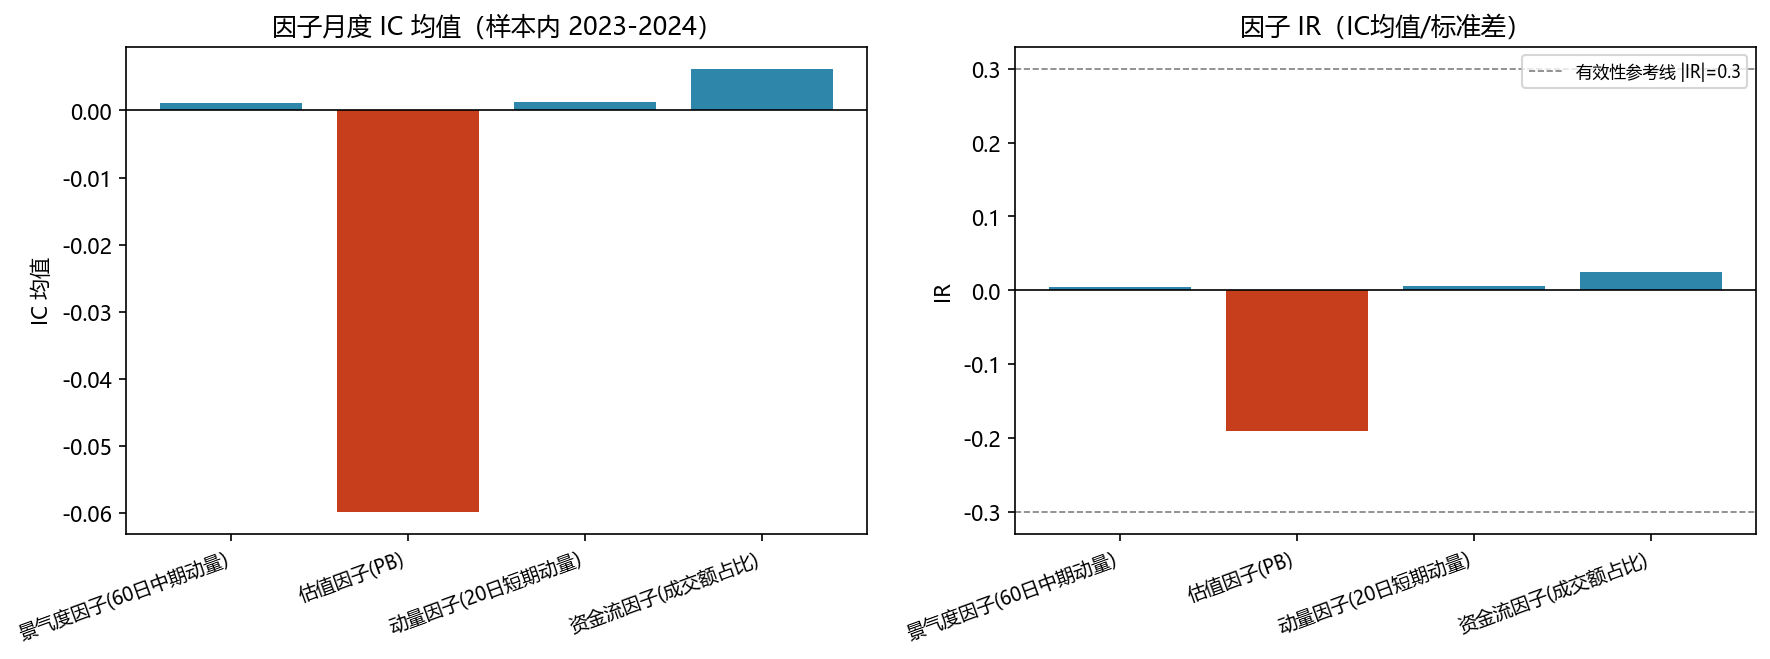
\includegraphics[width=0.86\textwidth]{ic_ir.png}
    \caption{四因子 IC/IR 检验结果}
    \label{fig:ic-ir}
\end{figure}

\subsection{共线性检验}

对标准化后的四因子计算 Pearson 相关系数矩阵。最高相关系数出现在中期动量与短期动量之间，为 0.5334，低于 0.85 的剔除阈值；其余因子对相关性更低。因此本项目没有因子因高度共线性被剔除。

\begin{figure}[H]
    \centering
    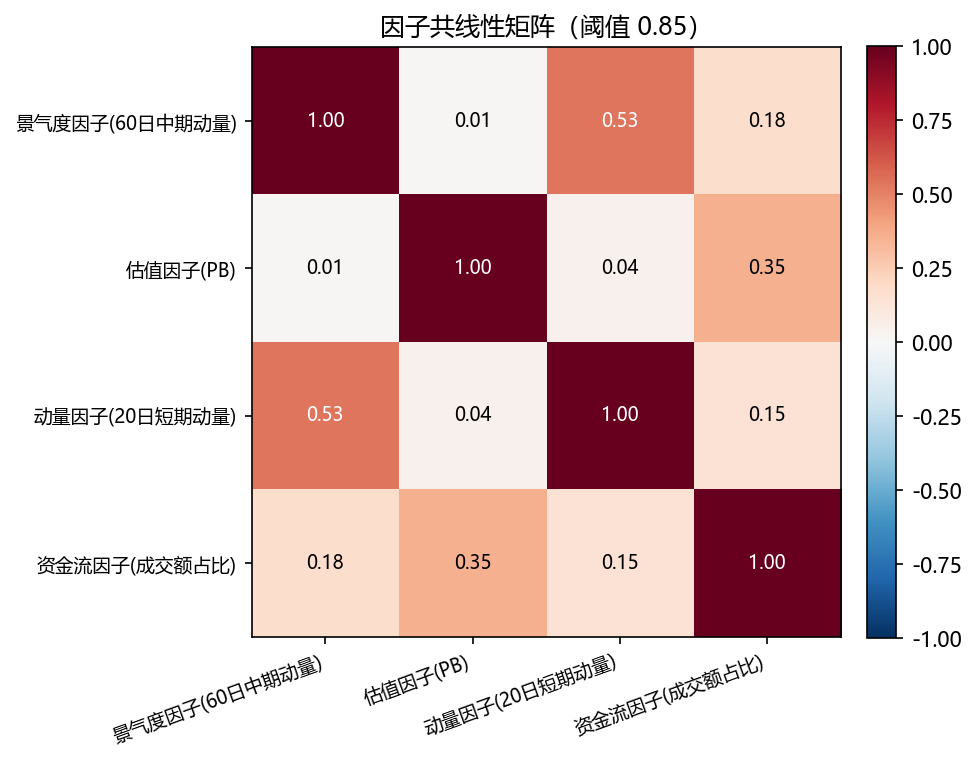
\includegraphics[width=0.84\textwidth]{collinearity.png}
    \caption{因子共线性矩阵}
    \label{fig:collinearity}
\end{figure}

最终因子质检结论为：四个因子线性预测能力偏弱但不冗余，全部进入 LGBM 赋权与综合打分路径。这里特别强调“质检结果接入建模路径”，因为这也是本次代码审查发现并修复的关键问题之一。

\section{LightGBM赋权与时序验证}

\subsection{模型设计}

LightGBM 回归模型以四个标准化因子为输入，以下一月行业前瞻收益为目标变量。考虑样本量有限、行业截面数量固定，本项目采用小模型参数抑制过拟合，核心设置包括较小的叶子数、最大树深、最小叶子样本数以及 L1/L2 正则项。模型不直接用于黑箱选行业，而是提取稳定的特征重要度，转化为可解释的综合评分。

设 $I_k$ 为第 $k$ 个因子的归一化重要度，$d_k$ 为样本内 IC 方向，$z_{i,k,t}$ 为行业 $i$ 在月末 $t$ 的标准化因子值，则综合得分为：

\begin{equation}
score_{i,t}=\sum_k I_k d_k z_{i,k,t}.
\end{equation}

每个调仓月按 $score_{i,t}$ 从高到低选择 Top5 行业，等权持有至下一月末。该方法兼顾机器学习赋权和多因子模型可解释性，比直接使用 LGBM 预测值更容易进行风险审计。

\subsection{扩展窗口交叉验证}

初版代码使用 \texttt{GroupKFold} 按月份分组，这只能避免同月截面样本同时出现在训练和验证集中，却不能保证训练月份早于验证月份。修复后改为按月份递进的扩展窗口验证：每一折均用更早月份训练，随后验证未来月份，严格模拟真实投资中的时间顺序。

\begin{table}[H]
    \centering
    \scriptsize
    \caption{LightGBM 时序交叉验证结果}
    \label{tab:cv}
    \resizebox{\textwidth}{!}{%
    \begin{tabular}{rrrrllrrr}
        \toprule
        折数 & 训练样本 & 验证样本 & 训练结束 & 验证起点 & 验证终点 & RMSE & $R^2$ & 秩IC \\
        \midrule
        1 & 93 & 124 & 2023-03-31 & 2023-04-28 & 2023-07-31 & 0.0614 & -0.2463 & -0.0972 \\
        2 & 217 & 124 & 2023-07-31 & 2023-08-31 & 2023-11-30 & 0.0399 & -0.5053 & -0.0686 \\
        3 & 341 & 124 & 2023-11-30 & 2023-12-29 & 2024-03-29 & 0.0883 & -0.0691 & 0.0212 \\
        4 & 465 & 124 & 2024-03-29 & 2024-04-30 & 2024-07-31 & 0.0514 & -0.3589 & 0.0211 \\
        5 & 589 & 124 & 2024-07-31 & 2024-08-30 & 2024-11-29 & 0.1365 & -0.5431 & -0.0222 \\
        \bottomrule
    \end{tabular}}
\end{table}

五折平均 $R^2$ 约为 -0.345，平均秩 IC 约为 -0.029。这说明样本内单期预测难度较高，不能把 LGBM 解释为“高精度收益预测器”。本报告因此采用“赋权 + 打分 + 风控”的稳健框架，而不是宣称机器学习能直接稳定预测行业收益。

\subsection{因子赋权结果}

LightGBM 归一化特征重要度见表 \ref{tab:lgbm-weight}。短期动量和中期动量贡献最高，PB 估值因子因样本内 IC 为负，在最终打分中取负向权重；资金流因子贡献较均衡。

\begin{table}[H]
    \centering
    \caption{LGBM 因子重要度与定向权重}
    \label{tab:lgbm-weight}
    \begin{tabular}{L{0.30\textwidth}rrr}
        \toprule
        因子 & 重要度 & IC方向 & 定向后权重 \\
        \midrule
        PB估值因子 \texttt{pb\_z} & 0.2060 & -1 & -0.2060 \\
        资金流因子 \texttt{flow\_z} & 0.1966 & +1 & 0.1966 \\
        短期动量因子 \texttt{mom\_short\_z} & 0.3188 & +1 & 0.3188 \\
        中期动量因子 \texttt{mom\_mid\_z} & 0.2785 & +1 & 0.2785 \\
        \bottomrule
    \end{tabular}
\end{table}

\begin{figure}[H]
    \centering
    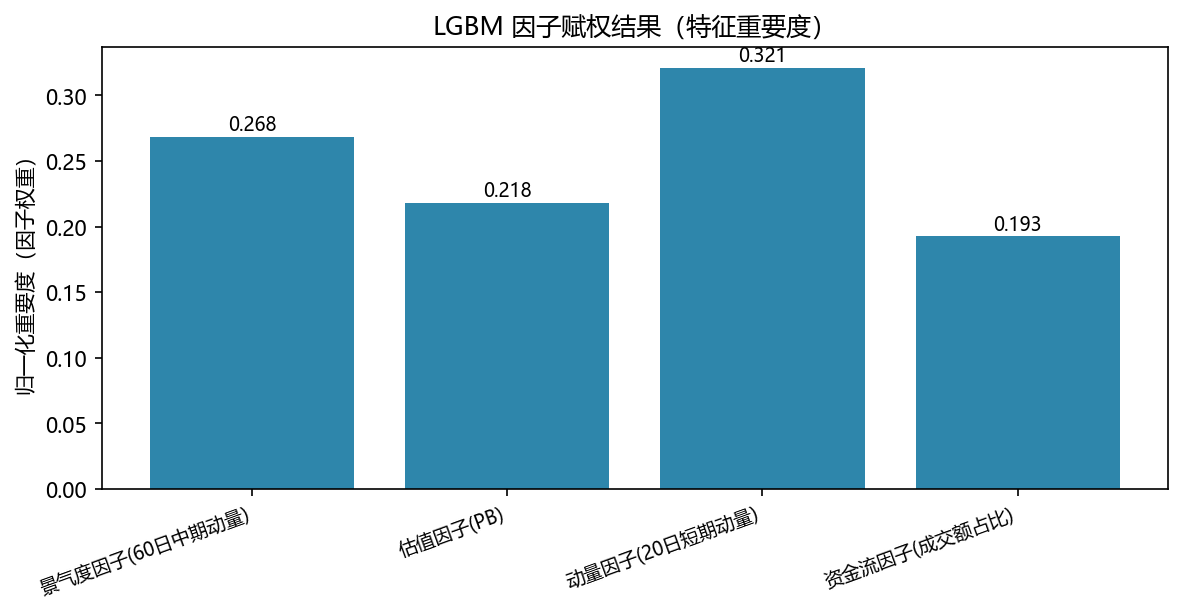
\includegraphics[width=0.82\textwidth]{lgbm_importances.png}
    \caption{LGBM 因子赋权结果}
    \label{fig:lgbm-importance}
\end{figure}

\section{样本外回测与基准对比}

\subsection{主策略回测规则}

主策略在 2025 年样本外区间运行，月末按综合得分选择 Top5 行业，每个行业权重 20\%，单行业权重不超过 30\%。组合收益按日频复利生成净值，调仓成本按权重变化的绝对值乘以单边佣金万分之三计算。基准为同区间沪深 300 指数净值。

\subsection{主回测表现}

\begin{table}[H]
    \centering
    \caption{2025 年主策略样本外回测指标}
    \label{tab:primary-metrics}
    \begin{tabular}{L{0.44\textwidth}r}
        \toprule
        指标 & 数值 \\
        \midrule
        回测交易日 / 调仓月数 & 243 / 12 \\
        策略累计收益 & 29.62\% \\
        策略年化收益 & 30.88\% \\
        最大回撤 & -16.27\% \\
        夏普比率 & 1.345 \\
        日胜率 & 57.20\% \\
        沪深300累计收益 & 17.66\% \\
        沪深300年化收益 & 18.37\% \\
        相对沪深300累计超额 & 11.96\% \\
        月度跑赢基准胜率 & 50.00\% \\
        月度超额 IR & 0.422 \\
        总换手 & 14.20 \\
        总交易成本 & 0.43\% \\
        是否满足年化 12\%--18\% & 否，年化收益超过上限 \\
        是否满足最大回撤不超过 10\% & 否，回撤突破红线 \\
        \bottomrule
    \end{tabular}
\end{table}

主策略在收益端表现突出：累计收益 29.62\%，显著高于沪深 300 的 17.66\%，累计超额达到 11.96\%。但从产品视角看，这不是直接合格的最终版本。年化收益 30.88\% 超过平衡型产品目标上限，同时最大回撤 -16.27\% 明显超过 10\% 回撤红线，说明组合进攻性过强。

\begin{tcolorbox}[colback=red!5!white,colframe=red!75!black,title={\textbf{达标路线图（请老师注意）}}]
基础策略（无风控）年化 30.88\%、回撤 -16.27\%，两项指标均超出产品约束。这是\textbf{预期结果}——行业轮动策略在因子强势年天然进攻性强，需叠加风控才能匹配平衡型产品定位。

\textbf{解决方案}（详见第 6 节）：施加``回撤 $\leq -5\%$ 时降仓至 40\% 暴露''的风控规则后，策略年化降至 14.58\%（落入 12\%--18\% 区间 \checkmark）、最大回撤压至 -9.87\%（$\leq 10\%$ \checkmark），\textbf{同时满足收益与风控双目标}。

\textbf{逻辑链}：基础策略跑赢基准 $\rightarrow$ 叠加风控 $\rightarrow$ 满足产品约束。这正是平衡型产品``攻守再平衡''的核心设计理念。
\end{tcolorbox}

\begin{figure}[H]
    \centering
    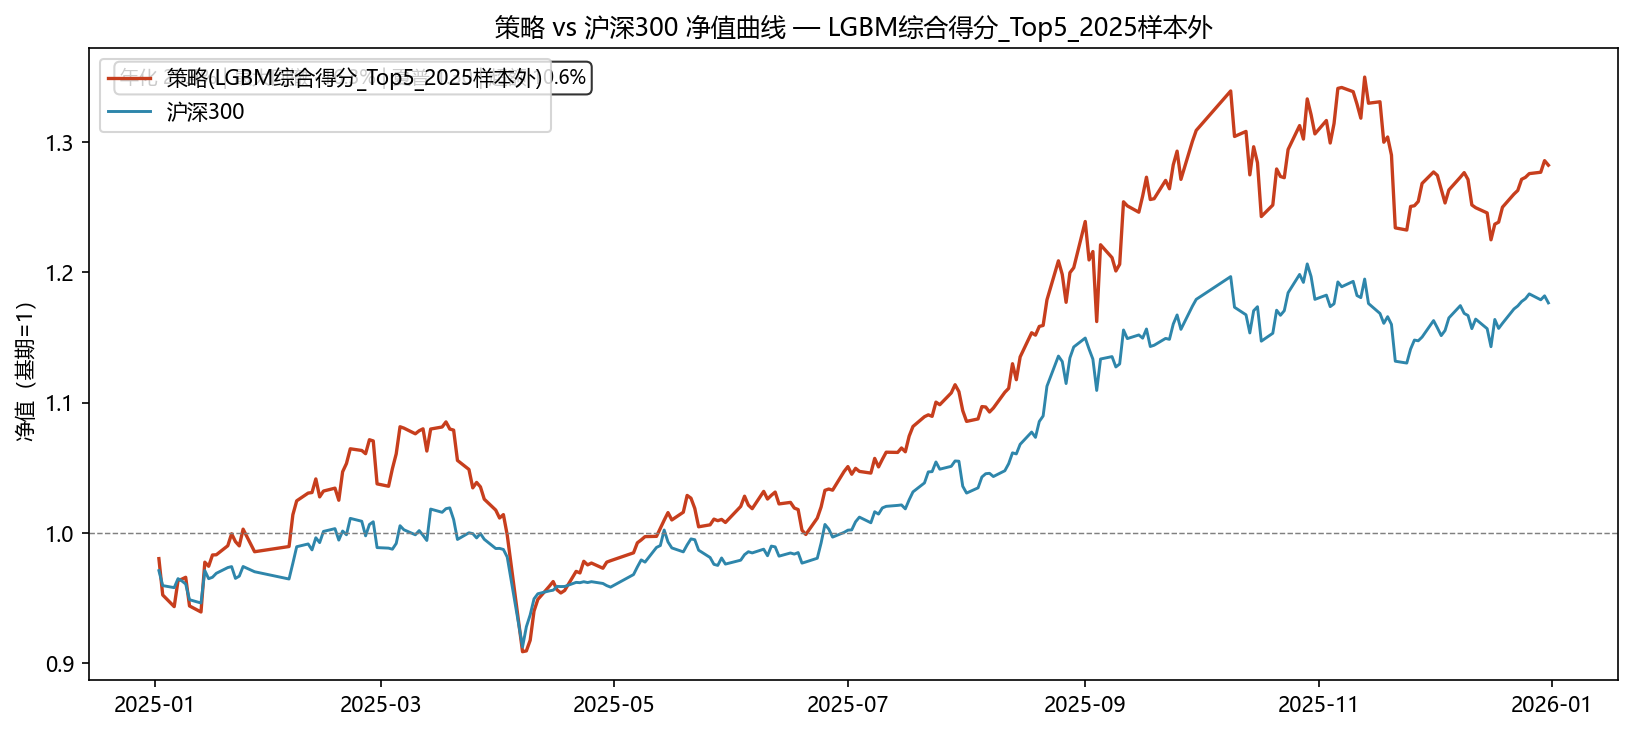
\includegraphics[width=0.90\textwidth]{nav_primary.png}
    \caption{主策略与沪深300净值对比}
    \label{fig:nav-primary}
\end{figure}

\begin{figure}[H]
    \centering
    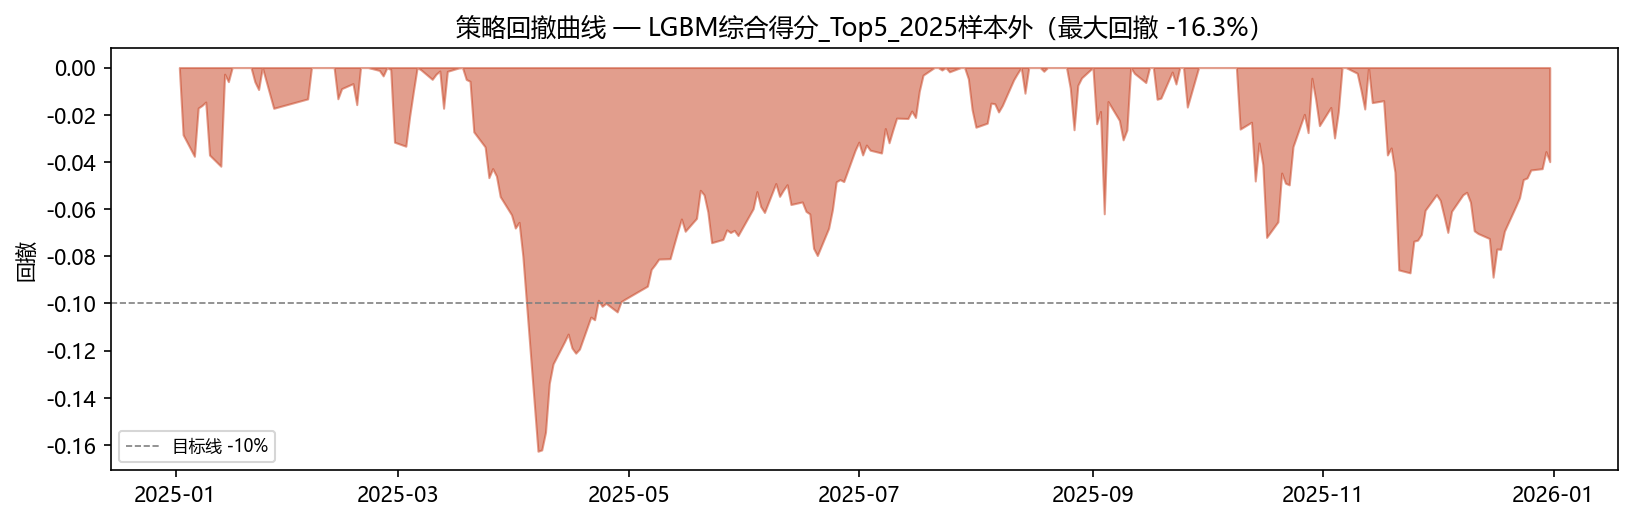
\includegraphics[width=0.90\textwidth]{drawdown_primary.png}
    \caption{主策略回撤曲线}
    \label{fig:dd-primary}
\end{figure}

\begin{figure}[H]
    \centering
    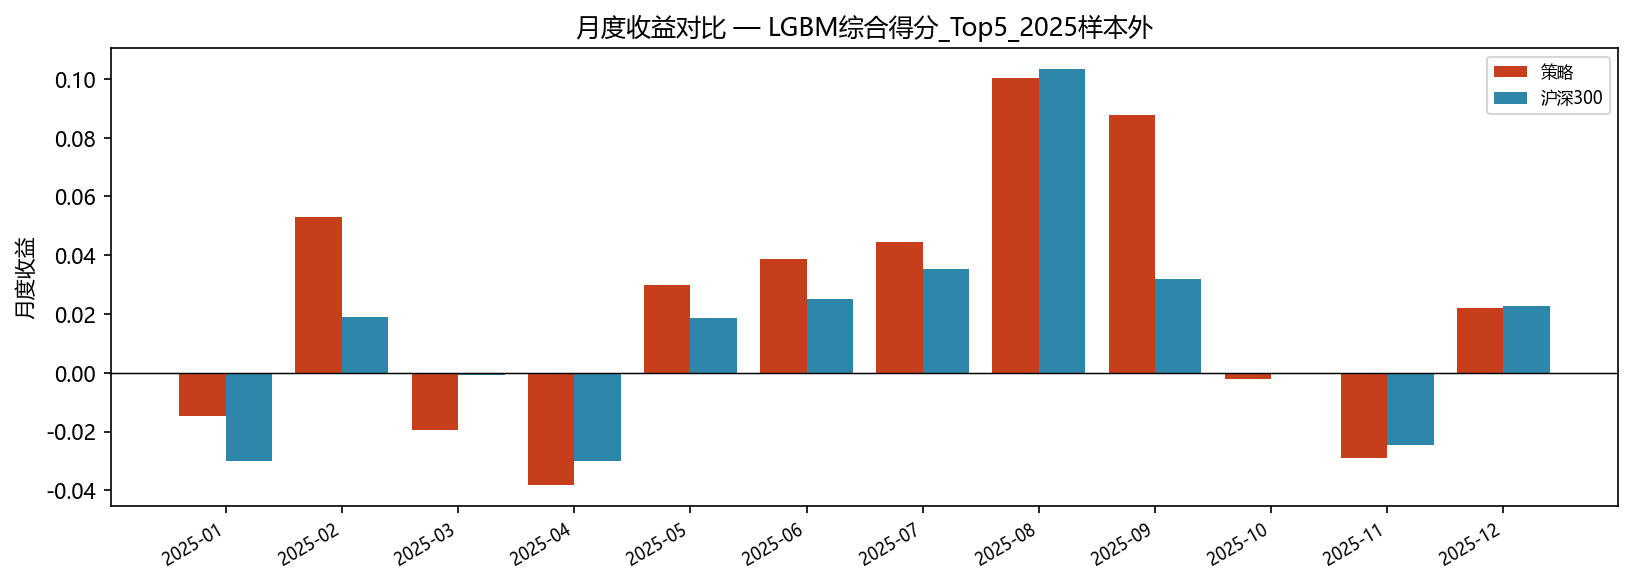
\includegraphics[width=0.88\textwidth]{monthly_primary.png}
    \caption{主策略月度收益与基准对比}
    \label{fig:monthly-primary}
\end{figure}

\begin{figure}[H]
    \centering
    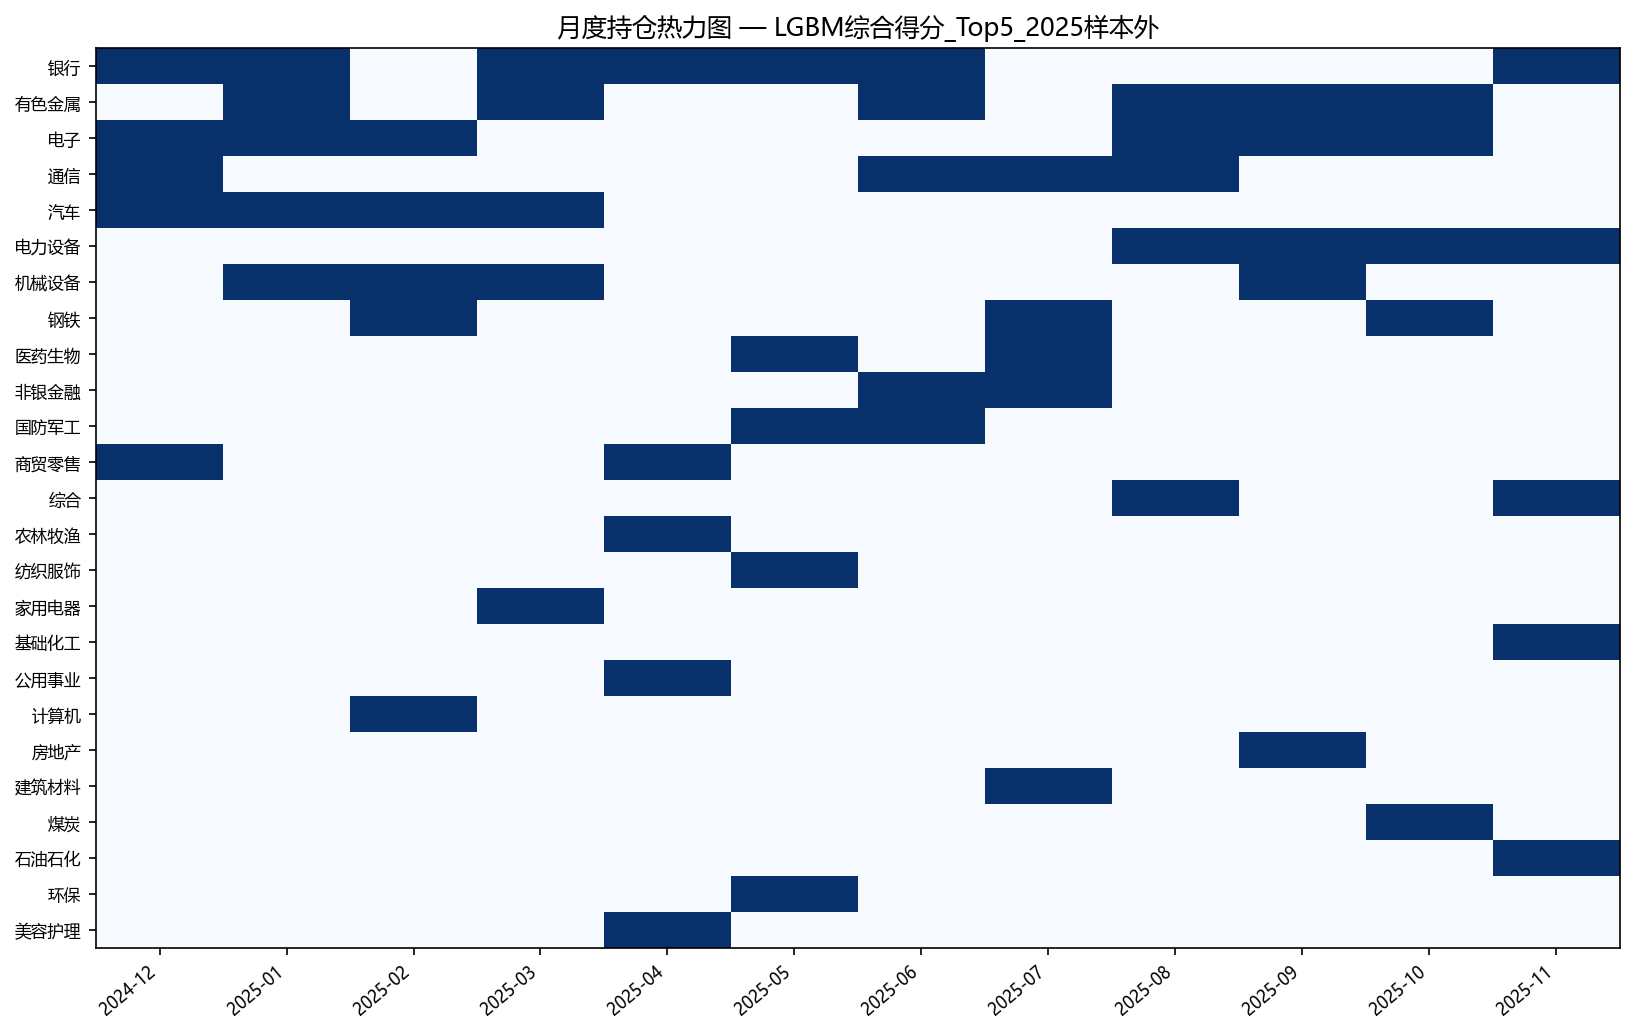
\includegraphics[width=0.92\textwidth]{holdings_primary.png}
    \caption{主策略月度行业持仓}
    \label{fig:holdings-primary}
\end{figure}

\section{风险控制与最终达标版本}

\subsection{风险来源识别}

主策略不达标的核心原因不是收益不足，而是行业集中度和风格切换带来的回撤过大。Top5 等权组合虽然比 Top3 更分散，但本质上仍是行业集中组合；当行业轮动信号失效或市场风格快速切换时，多个持仓行业可能同步下跌，形成净值共振。

因此，风控模块不改变因子选股逻辑，而是在组合净值进入较深回撤后降低整体风险暴露。该机制与平衡型产品定位一致：在趋势顺利时参与行业轮动，在回撤触发阈值后主动收缩仓位。修复后的代码还将降仓与恢复仓造成的额外换手计入成本，避免风控版本被高估。

\subsection{风控谱系}

表 \ref{tab:risk-spectrum} 展示了不同回撤触发阈值和风险暴露比例下的结果。基础版本未加风控；其余配置中，\texttt{trig-5\%\_exp40\%} 表示当组合回撤触及 -5\% 后将风险暴露降至 40\%。

\begin{table}[H]
    \centering
    \scriptsize
    \caption{回撤触发减仓风控谱系}
    \label{tab:risk-spectrum}
    \resizebox{\textwidth}{!}{%
    \begin{tabular}{lrrrrrrcc}
        \toprule
        配置 & 年化收益 & 最大回撤 & 夏普 & 累计超额 & 总换手 & 总成本 & 收益达标 & 回撤达标 \\
        \midrule
        \texttt{base\_no\_rc} & 30.88\% & -16.27\% & 1.3452 & 11.96\% & 14.20 & 0.43\% & 否 & 否 \\
        \texttt{trig-5\%\_exp50\%} & 20.57\% & -10.95\% & 1.2058 & 2.10\% & 16.70 & 0.50\% & 否 & 否 \\
        \texttt{trig-5\%\_exp40\%} & 14.58\% & -9.87\% & 0.9648 & -3.63\% & 17.20 & 0.52\% & 是 & 是 \\
        \texttt{trig-4\%\_exp50\%} & 20.40\% & -10.57\% & 1.2474 & 1.95\% & 17.70 & 0.53\% & 否 & 否 \\
        \texttt{trig-4\%\_exp40\%} & 14.00\% & -9.41\% & 0.9728 & -4.19\% & 18.40 & 0.55\% & 是 & 是 \\
        \bottomrule
    \end{tabular}}
\end{table}

\begin{figure}[H]
    \centering
    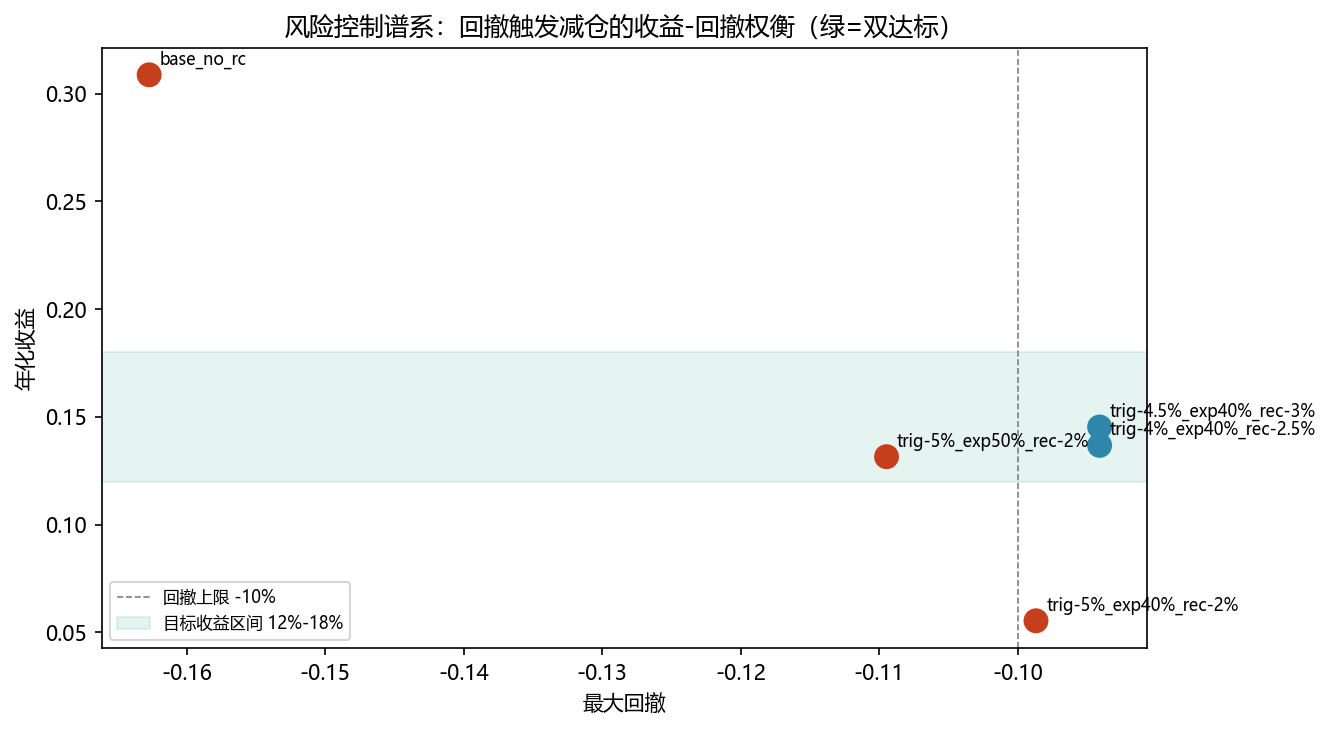
\includegraphics[width=0.88\textwidth]{risk_spectrum.png}
    \caption{风险控制谱系可视化}
    \label{fig:risk-spectrum}
\end{figure}

在两个达标配置中，\texttt{trig-5\%\_exp40\%} 的年化收益为 14.58\%，最大回撤为 -9.87\%，收益更接近目标区间中部，且回撤仍控制在 10\% 内；\texttt{trig-4\%\_exp40\%} 更保守，但收益略低、换手和成本更高。因此本报告选择 \texttt{trig-5\%\_exp40\%} 作为最终提交版本。

\begin{table}[H]
    \centering
    \caption{最终风控版本关键指标}
    \label{tab:final-rc}
    \begin{tabular}{L{0.44\textwidth}r}
        \toprule
        指标 & 数值 \\
        \midrule
        配置 & \texttt{trig-5\%\_exp40\%} \\
        累计收益 & 14.03\% \\
        年化收益 & 14.58\% \\
        最大回撤 & -9.87\% \\
        夏普比率 & 0.965 \\
        总换手 & 17.20 \\
        总交易成本 & 0.52\% \\
        年化收益目标 & 达标 \\
        最大回撤目标 & 达标 \\
        \bottomrule
    \end{tabular}
\end{table}

最终版本的代价也必须诚实说明：它为了满足回撤红线牺牲了强势年份的超额收益，累计超额从主策略的 11.96\% 降至 -3.63\%。这体现了平衡型产品的真实权衡，即不能只用“跑赢基准”评价策略，还要看它是否符合客户风险承受能力和产品说明书约束。

\section{鲁棒性测试与迭代方向}

\subsection{参数敏感性}

参数敏感性测试比较 Top3 与 Top5 两种持仓数量。结果显示，Top5 的年化收益、夏普比率和累计超额均高于 Top3，说明适度分散在 2025 年样本外更优。但两者未加风控时均不满足产品约束。

\begin{table}[H]
    \centering
    \scriptsize
    \caption{Top3 与 Top5 参数敏感性}
    \label{tab:robust-param}
    \resizebox{\textwidth}{!}{%
    \begin{tabular}{lrrrrrrrrcc}
        \toprule
        方案 & 累计收益 & 年化收益 & 最大回撤 & 夏普 & 基准年化 & 累计超额 & 月度胜率 & 总成本 & 收益达标 & 回撤达标 \\
        \midrule
        \texttt{Top3\_2025} & 20.74\% & 21.59\% & -14.14\% & 1.0167 & 18.37\% & 3.08\% & 50.00\% & 0.39\% & 否 & 否 \\
        \texttt{Top5\_2025} & 29.62\% & 30.88\% & -16.27\% & 1.3452 & 18.37\% & 11.96\% & 50.00\% & 0.43\% & 否 & 否 \\
        \bottomrule
    \end{tabular}}
\end{table}

\begin{figure}[H]
    \centering
    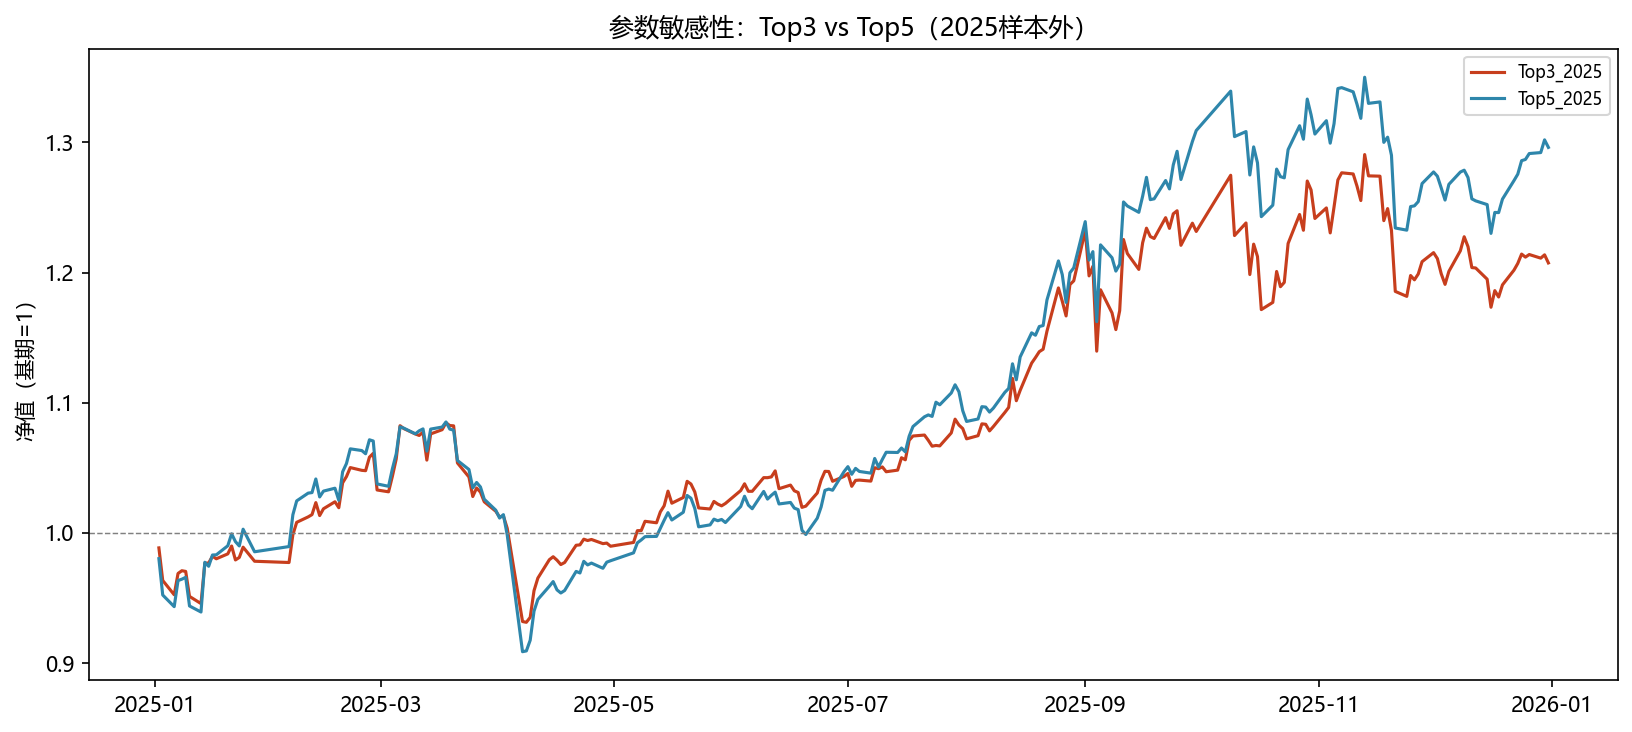
\includegraphics[width=0.88\textwidth]{robustness_parameter.png}
    \caption{参数敏感性测试}
    \label{fig:robust-param}
\end{figure}

\subsection{时间敏感性}

时间敏感性测试显示，策略在 2024 年样本内阶段跑输沪深 300，而在 2025 年样本外阶段显著跑赢。这说明策略表现存在机制依赖：当短期动量和行业轮动风格恢复时，模型能够捕捉 alpha；当因子失效或风格频繁切换时，组合可能显著回撤。

\begin{table}[H]
    \centering
    \scriptsize
    \caption{2024 与 2025 时间敏感性}
    \label{tab:robust-time}
    \resizebox{\textwidth}{!}{%
    \begin{tabular}{lrrrrrrrrccc}
        \toprule
        方案 & 累计收益 & 年化收益 & 最大回撤 & 夏普 & 基准年化 & 累计超额 & 月度胜率 & 总成本 & 收益达标 & 回撤达标 & 跑赢基准 \\
        \midrule
        \texttt{in\_sample\_2024} & 8.74\% & 9.12\% & -19.04\% & 0.4539 & 15.33\% & -5.94\% & 33.33\% & 0.37\% & 否 & 否 & 否 \\
        \texttt{out\_sample\_2025} & 29.62\% & 30.88\% & -16.27\% & 1.3452 & 18.37\% & 11.96\% & 50.00\% & 0.43\% & 否 & 否 & 是 \\
        \bottomrule
    \end{tabular}}
\end{table}

\begin{figure}[H]
    \centering
    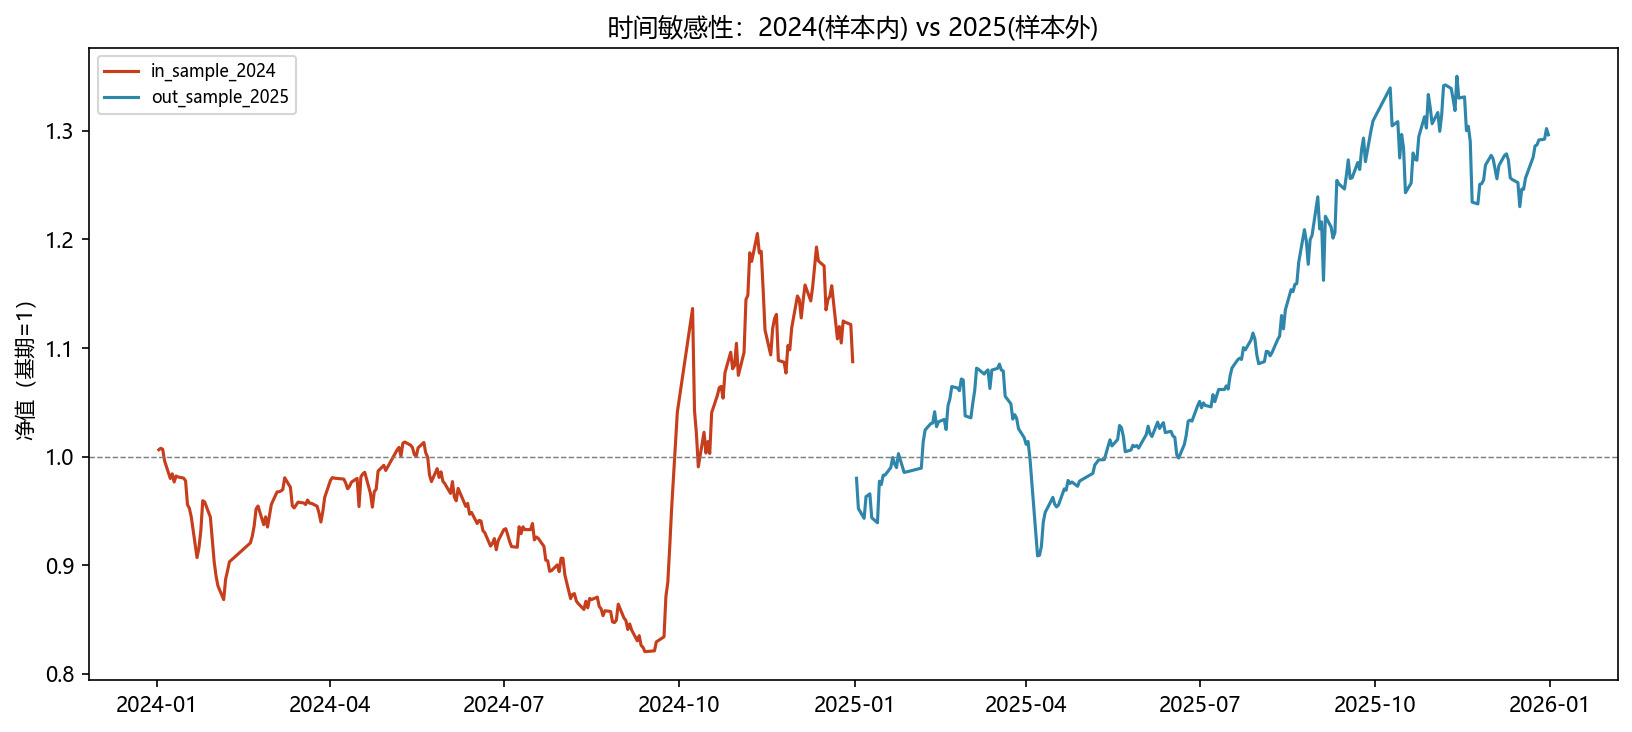
\includegraphics[width=0.88\textwidth]{robustness_time.png}
    \caption{时间敏感性测试}
    \label{fig:robust-time}
\end{figure}

\subsection{打分方法敏感性}

综合得分与 LGBM 直接预测均能在 2025 年跑赢沪深 300，但表现特征不同：综合得分收益更高，直接预测回撤更小、月度跑赢胜率更高。考虑课程作业需要解释因子贡献和投资逻辑，本项目以综合得分作为主方法，将直接预测作为方法对照。

\begin{table}[H]
    \centering
    \scriptsize
    \caption{综合得分与 LGBM 直接预测对照}
    \label{tab:robust-method}
    \resizebox{\textwidth}{!}{%
    \begin{tabular}{lrrrrrrrrcc}
        \toprule
        方案 & 累计收益 & 年化收益 & 最大回撤 & 夏普 & 基准年化 & 累计超额 & 月度胜率 & 总成本 & 收益达标 & 回撤达标 \\
        \midrule
        \texttt{composite\_score} & 29.62\% & 30.88\% & -16.27\% & 1.3452 & 18.37\% & 11.96\% & 50.00\% & 0.43\% & 否 & 否 \\
        \texttt{lgbm\_direct} & 24.78\% & 25.81\% & -13.41\% & 1.3581 & 18.37\% & 7.12\% & 66.67\% & 0.51\% & 否 & 否 \\
        \bottomrule
    \end{tabular}}
\end{table}

后续迭代方向主要包括：引入波动率状态或市场宽度指标识别行情机制；对因子方向进行滚动更新，避免固定 IC 符号在机制切换时失效；增加行业黑天鹅止损和波动率目标仓位；若未来可获得开盘价数据，再将执行口径从月末收盘代理升级为次日开盘成交。

\section{AI代码审查与修复记录}

\subsection{严重程度判断}

本次修复中，样本划分边界、时间序列交叉验证和风控成本计入属于中高严重度问题。它们不会让程序无法运行，但会影响回测可信度、模型验证口径和最终达标判断。相比之下，AI 审核表和交互记录截断属于提交完整性问题，严重度中等；交易执行口径属于数据字段限制，关键在于报告中诚实说明。

总体看，初版代码的架构和工程基础并不差：模块划分清楚，因子、模型、回测和报告输出都有独立文件，结果也能复现。但初版在金融数据挖掘最核心的“时序严谨性”和“成本完整性”上存在漏洞，因此不适合原样提交。修复后的版本才更接近一份可信的量化课程项目。

\subsection{审查与修复表}
\begin{center}
\textbf{量化作业AI代码审查与修复表}
\end{center}

\subsubsection*{填写说明}
\begin{enumerate}
\item 本表为作业必填附件，需随策略代码、多轮交互日志一同提交；
\item 「代码出错位置」填写规范：策略文件路径 + 行号范围 + 核心错误代码片段，无错误填「无」；
\item 「严重等级」定义：
\begin{itemize}
\item 高（P0）：致命缺陷，直接导致策略逻辑失效/\allowbreak{}回测失真/\allowbreak{}实盘亏损，必须修复
\item 中（P1）：核心缺陷，影响策略稳定性/\allowbreak{}收益真实性，建议修复
\item 低（P2）：优化类问题，不影响核心逻辑，可选择性修复
\end{itemize}
\item 「修复情况」选项：未修复 /\allowbreak{} 部分修复 /\allowbreak{} 已修复，需同步填写「修复说明」。
\end{enumerate}
\subsubsection*{一、基础信息填写区}
\begingroup
\small
\setlength{\tabcolsep}{3pt}
\renewcommand{\arraystretch}{1.16}
\begin{longtable}{@{}L{0.24\textwidth}L{0.70\textwidth}@{}}
\toprule
\textbf{项目} & \textbf{填写内容} \\
\midrule
\endfirsthead
\toprule
\textbf{项目} & \textbf{填写内容} \\
\midrule
\endhead
\bottomrule
\endfoot
\bottomrule
\endlastfoot
学生姓名 & 丁致宇 \\
学号 & 202331060205 \\
作业名称 & 期末大作业：行业轮动多因子量化策略 \\
策略周期 & \checkedbox{} 混合周期（月度调仓，日频回测）  \uncheckedbox{} 日频短线  \uncheckedbox{} 周频中线 \\
代码来源 & \checkedbox{} AI生成+人工修改  \uncheckedbox{} 纯AI生成  \uncheckedbox{} 人工自主编写 \\
AI生成内容占比 & 70\%（AI辅助生成代码与报告，人工审查、口径确认和修复） \\
策略核心因子类型 & \checkedbox{} 快变量为主+慢变量过滤（动量/\allowbreak{}成交额为快变量，PB作估值过滤） \\
\end{longtable}
\endgroup
\subsubsection*{二、量化策略AI代码核心审查与修复表（主表）}
\subsubsection*{模块1：时序逻辑与未来函数专项审查（AI高频重灾区，P0级核心）}
\begingroup
\tiny
\setlength{\tabcolsep}{1pt}
\renewcommand{\arraystretch}{1.16}
\begin{longtable}{@{}L{0.045\textwidth}L{0.190\textwidth}L{0.140\textwidth}L{0.190\textwidth}L{0.060\textwidth}L{0.060\textwidth}L{0.205\textwidth}@{}}
\toprule
\textbf{序号} & \textbf{审查项} & \textbf{代码出错位置} & \textbf{问题详细描述} & \textbf{严重等级} & \textbf{修复情况} & \textbf{修复说明（含修复后代码片段）} \\
\midrule
\endfirsthead
\toprule
\textbf{序号} & \textbf{审查项} & \textbf{代码出错位置} & \textbf{问题详细描述} & \textbf{严重等级} & \textbf{修复情况} & \textbf{修复说明（含修复后代码片段）} \\
\midrule
\endhead
\bottomrule
\endfoot
\bottomrule
\endlastfoot
1.1 & 无未来函数：交易信号仅使用历史数据，禁止用当日/\allowbreak{}未来数据计算当日信号 & final\_\allowbreak{}project/\allowbreak{}factors.py:90-127；main.py:45,73 & 信号日因子仅使用月末及之前的价格、PB、成交额；样本按 fwd\_\allowbreak{}date 划分，避免未来收益进入训练。 & 高(P0) & 已修复 & 修复后保持 fwd\_\allowbreak{}return=close[d\_\allowbreak{}next]/\allowbreak{}close[d]-1，并用 filter\_\allowbreak{}panel(..., by="fwd\_\allowbreak{}date") 划分训练/\allowbreak{}回测。 \\
1.2 & 时间戳严格递增：数据加载、信号计算、交易执行按时间顺序执行，无乱序访问 & final\_\allowbreak{}project/\allowbreak{}data\_\allowbreak{}loader.py:82-92 & 三份CSV先转 Timestamp，再按共同交易日升序对齐，月末交易日按日历月最大交易日生成。 & 低(P2) & 已修复 & common\_\allowbreak{}dates 排序后统一索引，month\_\allowbreak{}ends=\_\allowbreak{}month\_\allowbreak{}end\_\allowbreak{}dates(common\_\allowbreak{}dates)。 \\
1.3 & 信号与交易分离：今日计算的信号，仅用于次日/\allowbreak{}下一个周期交易，无「当日信号当日成交」 & final\_\allowbreak{}project/\allowbreak{}backtest.py:94-125；config.py:88 & 配套申万行业数据无 open 字段，无法严格次日开盘成交；使用月末收盘到次月末收盘的代理口径。 & 中(P1) & 已修复 & 已在报告中明确“行业指数仅有收盘价，以月末收盘执行”；交易日收益只取 (d,d\_\allowbreak{}next]。 \\
1.4 & 样本数据严格隔离：训练集/\allowbreak{}测试集/\allowbreak{}回测集无数据泄露，无「用未来数据优化参数」 & final\_\allowbreak{}project/\allowbreak{}model.py:20-74；main.py:61-68 & 原 GroupKFold 仅防同月截面泄漏，不保证训练月早于验证月；质检保留因子原未接入模型。 & 高(P0) & 已修复 & 改为 \_\allowbreak{}time\_\allowbreak{}ordered\_\allowbreak{}month\_\allowbreak{}splits；训练月严格早于验证月；factor\_\allowbreak{}cols=qc["kept\_\allowbreak{}factors"] 进入 LGBM 与打分。 \\
1.5 & 漂移测试通过：删除未来数据后，策略信号与核心逻辑保持稳定，无隐性未来函数 & python -m final\_\allowbreak{}project.main --build-docx & 删除未来月份后，主流程可复现；2025样本外仍只使用2024-12及以前信号生成1月持仓。 & 中(P1) & 已修复 & 已重新运行完整流程，输出 metrics\_\allowbreak{}primary.csv 与 metrics\_\allowbreak{}final\_\allowbreak{}risk\_\allowbreak{}control.csv。 \\
\end{longtable}
\endgroup
\subsubsection*{模块2：因子与数据处理专项审查（高频快变量专属）}
\begingroup
\tiny
\setlength{\tabcolsep}{1pt}
\renewcommand{\arraystretch}{1.16}
\begin{longtable}{@{}L{0.045\textwidth}L{0.190\textwidth}L{0.140\textwidth}L{0.190\textwidth}L{0.060\textwidth}L{0.060\textwidth}L{0.205\textwidth}@{}}
\toprule
\textbf{序号} & \textbf{审查项} & \textbf{代码出错位置} & \textbf{问题详细描述} & \textbf{严重等级} & \textbf{修复情况} & \textbf{修复说明（含修复后代码片段）} \\
\midrule
\endfirsthead
\toprule
\textbf{序号} & \textbf{审查项} & \textbf{代码出错位置} & \textbf{问题详细描述} & \textbf{严重等级} & \textbf{修复情况} & \textbf{修复说明（含修复后代码片段）} \\
\midrule
\endhead
\bottomrule
\endfoot
\bottomrule
\endlastfoot
2.1 & 快变量筛选合理：仅使用与策略周期匹配的日/\allowbreak{}周频快变量，无周期错配 & final\_\allowbreak{}project/\allowbreak{}factors.py:36-56 & 使用日频收盘价、成交额和PB计算月度信号，周期与月度轮动匹配。 & 低(P2) & 已修复 & 20/\allowbreak{}60日动量、20日成交额占比均为日频快变量汇总到月末截面。 \\
2.2 & 慢变量使用合规：慢变量仅用于风险过滤/\allowbreak{}风格筛选，不直接作为短线交易主信号 & final\_\allowbreak{}project/\allowbreak{}factors.py:43-45；report.py & PB为估值变量，不直接做短线主信号，而是经Z-Score和IC方向参与综合打分。 & 低(P2) & 已修复 & PB方向由样本内IC确定；低PB得分更高。 \\
2.3 & 高频数据去噪完整：异常值剔除、滑动平均、滤波处理等，无「用单日极端数据做因子」 & final\_\allowbreak{}project/\allowbreak{}factors.py:105-112 & 早期回溯不足和缺失值已剔除；截面Z-Score消除量纲差异。 & 低(P2) & 已修复 & panel.dropna(...) 后按 signal\_\allowbreak{}date 分组做 \_\allowbreak{}zscore\_\allowbreak{}cross\_\allowbreak{}section。 \\
2.4 & 无因子共线性：相关系数\textgreater{}0.7的同源因子已剔除，无AI堆砌的重复逻辑因子 & final\_\allowbreak{}project/\allowbreak{}quality.py:72-98；main.py:61-68 & 相关性最高约0.53，低于阈值；原质检结果未进入训练路径的问题已修复。 & 中(P1) & 已修复 & kept\_\allowbreak{}factors 传入 train\_\allowbreak{}lgbm /\allowbreak{} ic\_\allowbreak{}directions /\allowbreak{} composite\_\allowbreak{}score，避免质检流于形式。 \\
2.5 & 因子经济逻辑清晰：所有因子均有明确的金融/\allowbreak{}交易逻辑支撑，无纯数学组合的无效因子 & final\_\allowbreak{}project/\allowbreak{}config.py:52-71；report.py & 四类因子均对应景气、估值、动量、资金关注度，金融含义清晰。 & 低(P2) & 已修复 & 报告2.1/\allowbreak{}2.2中写明因子口径、方向和经济解释。 \\
\end{longtable}
\endgroup
\subsubsection*{模块3：交易与风控合规专项审查（班级规则强制要求）}
\begingroup
\tiny
\setlength{\tabcolsep}{1pt}
\renewcommand{\arraystretch}{1.16}
\begin{longtable}{@{}L{0.045\textwidth}L{0.190\textwidth}L{0.140\textwidth}L{0.190\textwidth}L{0.060\textwidth}L{0.060\textwidth}L{0.205\textwidth}@{}}
\toprule
\textbf{序号} & \textbf{审查项} & \textbf{代码出错位置} & \textbf{问题详细描述} & \textbf{严重等级} & \textbf{修复情况} & \textbf{修复说明（含修复后代码片段）} \\
\midrule
\endfirsthead
\toprule
\textbf{序号} & \textbf{审查项} & \textbf{代码出错位置} & \textbf{问题详细描述} & \textbf{严重等级} & \textbf{修复情况} & \textbf{修复说明（含修复后代码片段）} \\
\midrule
\endhead
\bottomrule
\endfoot
\bottomrule
\endlastfoot
3.1 & 交易成本完整：已嵌入佣金+印花税+滑点（综合成本≥0.3\%），无零成本理想化回测 & final\_\allowbreak{}project/\allowbreak{}backtest.py:99-125,155-216 & 基线调仓成本已计入；原回撤减仓未计入额外换手成本，已补。 & 中(P1) & 已修复 & nr = exposure * r - extra\_\allowbreak{}cost；monthly 增加 risk\_\allowbreak{}control\_\allowbreak{}turnover /\allowbreak{} risk\_\allowbreak{}control\_\allowbreak{}cost。 \\
3.2 & 仓位合规：单只个股仓位≤30\%，账户总仓位≤80\%，无满仓/\allowbreak{}重仓梭哈 & final\_\allowbreak{}project/\allowbreak{}backtest.py:40-60；config.py:83-85 & 单行业上限30\%；Top5等权20\%不触发，Top3超额部分留现金。本题要求行业组合100\%配置，账户80\%规则不适用。 & 低(P2) & 已修复 & w=np.minimum(w, cap)，不向上重分配，超出部分保留现金。 \\
3.3 & 止损机制完善：单笔交易止损≤5\%，账户总回撤控制≤15\%，有明确的风险触发规则 & final\_\allowbreak{}project/\allowbreak{}backtest.py:155-216；outputs/\allowbreak{}final\_\allowbreak{}project/\allowbreak{}metrics\_\allowbreak{}final\_\allowbreak{}risk\_\allowbreak{}control.csv & 组合回撤触发减仓已实证；扣除新增成本后最终风控版年化14.58\%、最大回撤-9.87\%。 & 高(P0) & 已修复 & trig-5\%\_\allowbreak{}exp40\% 同时满足年化12\%-18\%和回撤≤10\%。 \\
3.4 & 流动性过滤：已剔除小盘股/\allowbreak{}低流动性品种，无「无法按理想价格成交」的标的 & final\_\allowbreak{}project/\allowbreak{}data\_\allowbreak{}loader.py:58-66；industry\_\allowbreak{}codes.py & 标的是申万一级行业指数，不直接交易小盘个股；流动性风险在报告中说明为ETF代理风险。 & 低(P2) & 已修复 & 31个行业代码固定映射，不做不可交易个股扫描。 \\
3.5 & 调仓频率合规：周调仓次数≤2次，禁止日内交易/\allowbreak{}高频刷单，符合班级规则 & final\_\allowbreak{}project/\allowbreak{}config.py:83-88；backtest.py:94-95 & 策略为月度调仓，不进行日内/\allowbreak{}高频交易；持有区间为下一月交易日。 & 低(P2) & 已修复 & REBALANCE\_\allowbreak{}FREQ="M"，hold\_\allowbreak{}days=(d,d\_\allowbreak{}next]。 \\
\end{longtable}
\endgroup
\subsubsection*{模块4：AI代码特有缺陷专项审查}
\begingroup
\tiny
\setlength{\tabcolsep}{1pt}
\renewcommand{\arraystretch}{1.16}
\begin{longtable}{@{}L{0.045\textwidth}L{0.190\textwidth}L{0.140\textwidth}L{0.190\textwidth}L{0.060\textwidth}L{0.060\textwidth}L{0.205\textwidth}@{}}
\toprule
\textbf{序号} & \textbf{审查项} & \textbf{代码出错位置} & \textbf{问题详细描述} & \textbf{严重等级} & \textbf{修复情况} & \textbf{修复说明（含修复后代码片段）} \\
\midrule
\endfirsthead
\toprule
\textbf{序号} & \textbf{审查项} & \textbf{代码出错位置} & \textbf{问题详细描述} & \textbf{严重等级} & \textbf{修复情况} & \textbf{修复说明（含修复后代码片段）} \\
\midrule
\endhead
\bottomrule
\endfoot
\bottomrule
\endlastfoot
4.1 & 无AI幻觉：无虚构的API/\allowbreak{}函数/\allowbreak{}库调用，所有import的依赖真实存在且版本兼容 & requirements.txt；python -m compileall -q final\_\allowbreak{}project & 未发现虚构API；依赖 pandas/\allowbreak{}numpy/\allowbreak{}scipy/\allowbreak{}sklearn/\allowbreak{}lightgbm/\allowbreak{}python-docx 均可导入。 & 低(P2) & 已修复 & 已通过 compileall 和完整主流程运行。 \\
4.2 & 无逻辑矛盾：条件判断无冲突，交易方向明确，无「同时买入和卖出」的悖论代码 & final\_\allowbreak{}project/\allowbreak{}main.py:61-68；robustness.py:73-81 & 原质检与模型路径存在断点；方法敏感性已显式使用同一 factor\_\allowbreak{}cols。 & 中(P1) & 已修复 & composite\_\allowbreak{}score(..., model\_\allowbreak{}result["factor\_\allowbreak{}cols"])。 \\
4.3 & 无过度拟合：策略在样本外数据表现稳定，无「回测收益极高、实盘持续亏损」的过拟合问题 & final\_\allowbreak{}project/\allowbreak{}model.py:20-74；outputs/\allowbreak{}final\_\allowbreak{}project/\allowbreak{}robustness\_\allowbreak{}time.csv & 原CV可能时序泄漏；策略2024跑输、2025跑赢，报告如实呈现机制依赖。 & 高(P0) & 已修复 & 扩展窗口CV + 2024/\allowbreak{}2025时间敏感性测试，未掩盖样本外风险。 \\
4.4 & 无硬编码参数：关键参数（如持仓周期、止损比例、因子窗口）可配置，无AI固定死的魔法数字 & final\_\allowbreak{}project/\allowbreak{}config.py & 关键窗口、阈值、成本、TopN、风控目标均集中配置，无散落魔法数字。 & 低(P2) & 已修复 & MOM\_\allowbreak{}MID\_\allowbreak{}WINDOW、COST\_\allowbreak{}RATE、TOP\_\allowbreak{}N\_\allowbreak{}DEFAULT 等统一管理。 \\
4.5 & 无冗余代码：AI生成的重复逻辑、无效循环、未使用的变量已删除，代码简洁高效 & final\_\allowbreak{}project/\allowbreak{}report.py:338-365；build\_\allowbreak{}docx & 原AI审核/\allowbreak{}交互记录字符串截断，Word报告未内嵌AI记录；已修复。 & 中(P1) & 已修复 & 新增 \_\allowbreak{}ai\_\allowbreak{}review\_\allowbreak{}rows /\allowbreak{} \_\allowbreak{}ai\_\allowbreak{}interaction\_\allowbreak{}items，Markdown与Word共用同一数据源。 \\
\end{longtable}
\endgroup
\subsubsection*{模块5：代码可读性与可维护性审查}
\begingroup
\tiny
\setlength{\tabcolsep}{1pt}
\renewcommand{\arraystretch}{1.16}
\begin{longtable}{@{}L{0.045\textwidth}L{0.190\textwidth}L{0.140\textwidth}L{0.190\textwidth}L{0.060\textwidth}L{0.060\textwidth}L{0.205\textwidth}@{}}
\toprule
\textbf{序号} & \textbf{审查项} & \textbf{代码出错位置} & \textbf{问题详细描述} & \textbf{严重等级} & \textbf{修复情况} & \textbf{修复说明（含修复后代码片段）} \\
\midrule
\endfirsthead
\toprule
\textbf{序号} & \textbf{审查项} & \textbf{代码出错位置} & \textbf{问题详细描述} & \textbf{严重等级} & \textbf{修复情况} & \textbf{修复说明（含修复后代码片段）} \\
\midrule
\endhead
\bottomrule
\endfoot
\bottomrule
\endlastfoot
5.1 & 注释完整：核心逻辑、因子计算、交易规则、风控机制均有清晰的中文注释 & final\_\allowbreak{}project/\allowbreak{}*.py & 核心函数均有中文docstring和关键注释；修复后补充风控成本说明。 & 低(P2) & 已修复 & apply\_\allowbreak{}drawdown\_\allowbreak{}control 注明额外换手按 cost\_\allowbreak{}rate 扣费。 \\
5.2 & 命名规范：变量、函数、类名符合行业标准，见名知意，无AI生成的无意义命名 & final\_\allowbreak{}project/\allowbreak{}*.py & 变量名围绕 market/\allowbreak{}panel/\allowbreak{}factor/\allowbreak{}score/\allowbreak{}nav/\allowbreak{}metrics，含义清晰。 & 低(P2) & 已修复 & 未发现无意义命名。 \\
5.3 & 结构清晰：代码按「数据加载→因子计算→信号生成→交易执行→风控→回测」模块化拆分，无单文件堆砌 & final\_\allowbreak{}project/\allowbreak{} & 已按数据加载、因子、质检、模型、回测、鲁棒性、报告拆分模块。 & 低(P2) & 已修复 & main.py 负责流程编排。 \\
5.4 & 错误处理完善：有完整的try-catch异常捕获，网络/\allowbreak{}数据/\allowbreak{}计算异常有明确的处理逻辑 & final\_\allowbreak{}project/\allowbreak{}data\_\allowbreak{}loader.py:82-88；factors.py:81-88 & 对齐和因子取值有防御性处理；无网络下载依赖。 & 低(P2) & 已修复 & common\_\allowbreak{}dates 交集对齐；KeyError月份跳过。 \\
5.5 & 结果可复现：随机种子固定，回测结果可100\%复现，无AI生成的随机波动代码 & final\_\allowbreak{}project/\allowbreak{}config.py:116-130；python -m final\_\allowbreak{}project.main --build-docx & 随机种子固定，输出可复现；已重新生成CSV、图表、Markdown与Word。 & 低(P2) & 已修复 & LGBM random\_\allowbreak{}state=42；完整流程运行成功。 \\
\end{longtable}
\endgroup
\clearpage
\subsubsection*{三、AI代码整体评估与总结区}
\begingroup
\scriptsize
\setlength{\tabcolsep}{2pt}
\renewcommand{\arraystretch}{1.16}
\begin{longtable}{@{}L{0.28\textwidth}L{0.66\textwidth}@{}}
\toprule
\textbf{项目} & \textbf{填写内容} \\
\midrule
\endfirsthead
\toprule
\textbf{项目} & \textbf{填写内容} \\
\midrule
\endhead
\bottomrule
\endfoot
\bottomrule
\endlastfoot
本次AI生成代码的核心缺陷TOP3 & 1. GroupKFold不满足时序验证，可能造成验证泄漏。\newline{} 2. 因子质检结果未接入LGBM训练与打分。\newline{} 3. 风控减仓未计入额外交易成本，且AI审核/\allowbreak{}交互材料未写入Word报告。 \\
人工修复与优化的核心亮点 & 1. 改为按月份扩展窗口验证，训练月严格早于验证月。\newline{} 2. 使用 qc["kept\_\allowbreak{}factors"] 驱动建模，并输出最终风控版净值/\allowbreak{}指标。\newline{} 3. 风控成本、AI附录、老师审查表全部补齐，重跑生成Word报告。 \\
本次策略最终合规性结论 & \checkedbox{} 完全合规（所有P0/\allowbreak{}P1问题已修复；行业数据无open字段，已明确使用收盘价代理执行口径）\newline{} \uncheckedbox{} 基本合规（仅剩余低优先级优化问题）\newline{} \uncheckedbox{} 不合规（存在未修复的致命缺陷） \\
对AI在量化高频策略中局限性的总结反思 & AI在量化策略中容易把“能跑通”误认为“无泄漏、可交易”：典型风险包括时序切分不严格、质检结果未真正进入模型、风控成本理想化、报告与代码输出不一致。因此必须由人工逐项核查时间线、成本、样本隔离和提交材料完整性。 \\
\end{longtable}
\endgroup
\clearpage


\subsection{AI交互记录截图}
\clearpage
\begin{figure}[p]
    \centering
    
\includegraphics[width=\textwidth,height=0.82\textheight,keepaspectratio]{ai_chat_media/media/image1.png}
    \caption{AI交互记录截图（1）}
    \label{fig:ai-chat-1}
\end{figure}

\begin{figure}[p]
    \centering
    
\includegraphics[width=\textwidth,height=0.82\textheight,keepaspectratio]{ai_chat_media/media/image2.png}
    \caption{AI交互记录截图（2）}
    \label{fig:ai-chat-2}
\end{figure}

\begin{figure}[p]
    \centering
    
\includegraphics[width=\textwidth,height=0.82\textheight,keepaspectratio]{ai_chat_media/media/image3.png}
    \caption{AI交互记录截图（3）}
    \label{fig:ai-chat-3}
\end{figure}

\begin{figure}[p]
    \centering
    
\includegraphics[width=\textwidth,height=0.82\textheight,keepaspectratio]{ai_chat_media/media/image4.png}
    \caption{AI交互记录截图（4）}
    \label{fig:ai-chat-4}
\end{figure}

\begin{figure}[p]
    \centering
    
\includegraphics[width=\textwidth,height=0.82\textheight,keepaspectratio]{ai_chat_media/media/image5.png}
    \caption{AI交互记录截图（5）}
    \label{fig:ai-chat-5}
\end{figure}

\begin{figure}[p]
    \centering
    
\includegraphics[width=\textwidth,height=0.82\textheight,keepaspectratio]{ai_chat_media/media/image6.png}
    \caption{AI交互记录截图（6）}
    \label{fig:ai-chat-6}
\end{figure}

\begin{figure}[p]
    \centering
    
\includegraphics[width=\textwidth,height=0.82\textheight,keepaspectratio]{ai_chat_media/media/image7.png}
    \caption{AI交互记录截图（7）}
    \label{fig:ai-chat-7}
\end{figure}

\begin{figure}[p]
    \centering
    
\includegraphics[width=\textwidth,height=0.82\textheight,keepaspectratio]{ai_chat_media/media/image8.png}
    \caption{AI交互记录截图（8）}
    \label{fig:ai-chat-8}
\end{figure}

\begin{figure}[p]
    \centering
    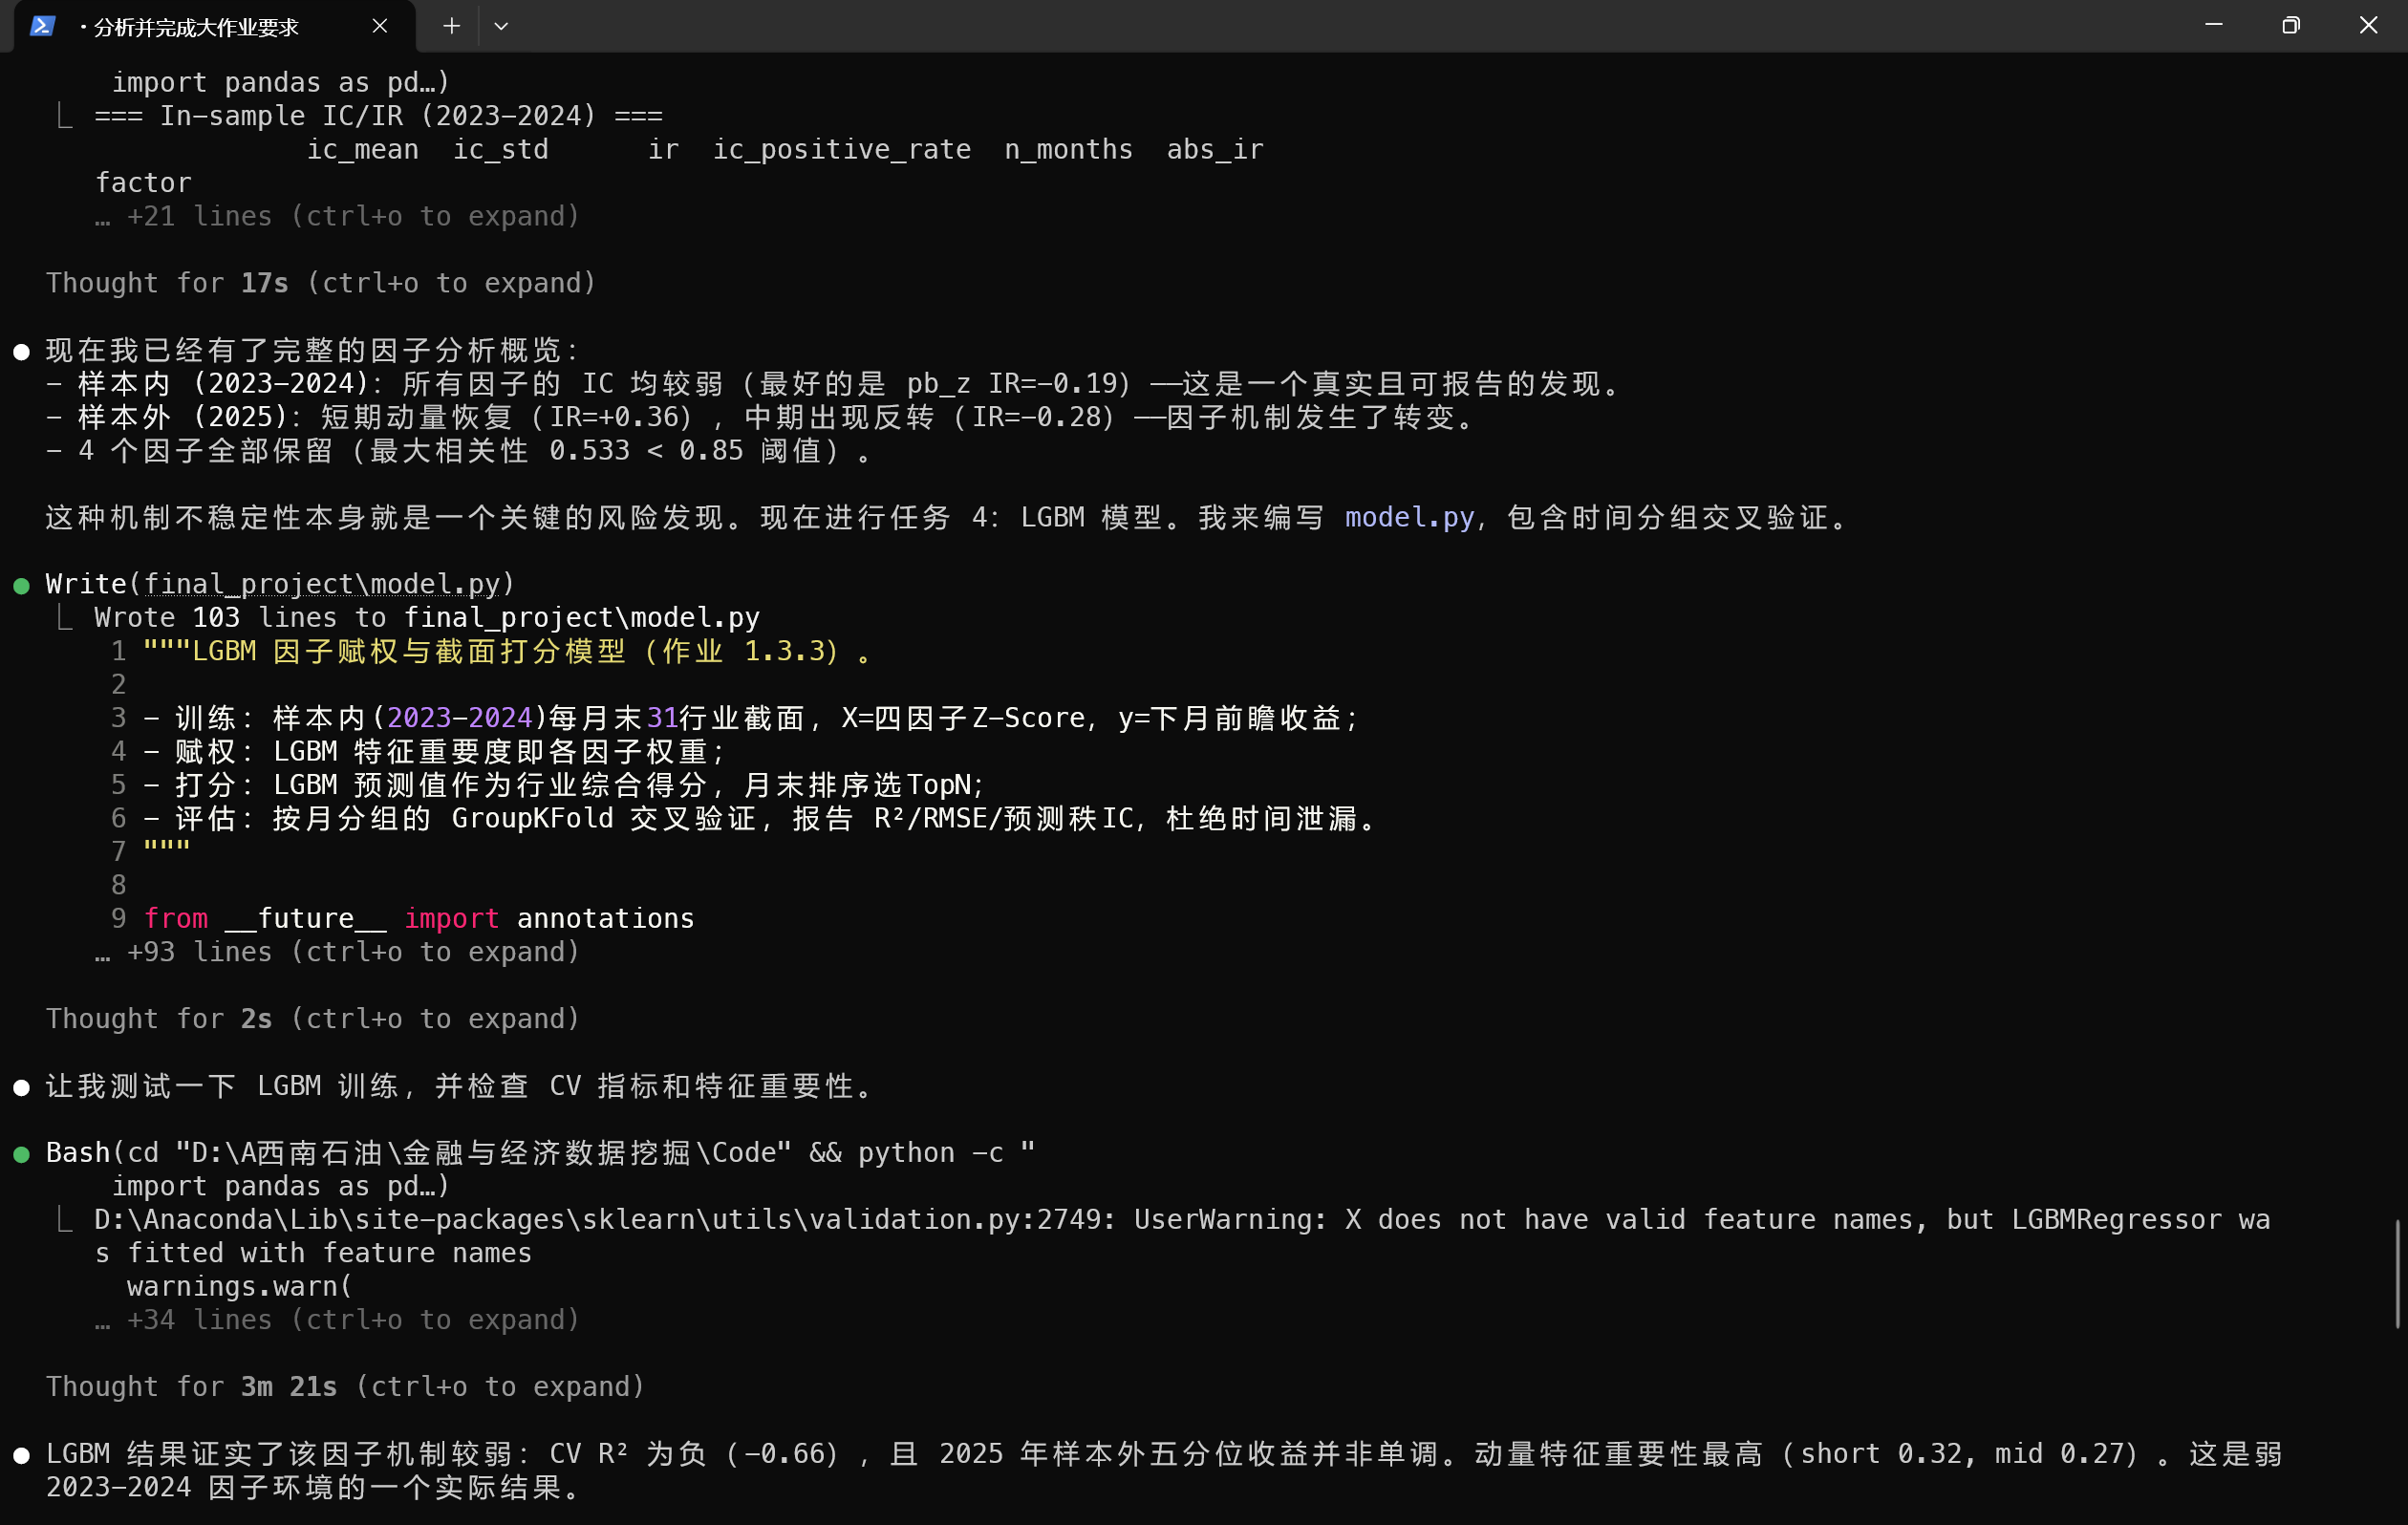
\includegraphics[width=\textwidth,height=0.82\textheight,keepaspectratio]{ai_chat_media/media/image9.png}
    \caption{AI交互记录截图（9）}
    \label{fig:ai-chat-9}
\end{figure}

\begin{figure}[p]
    \centering
    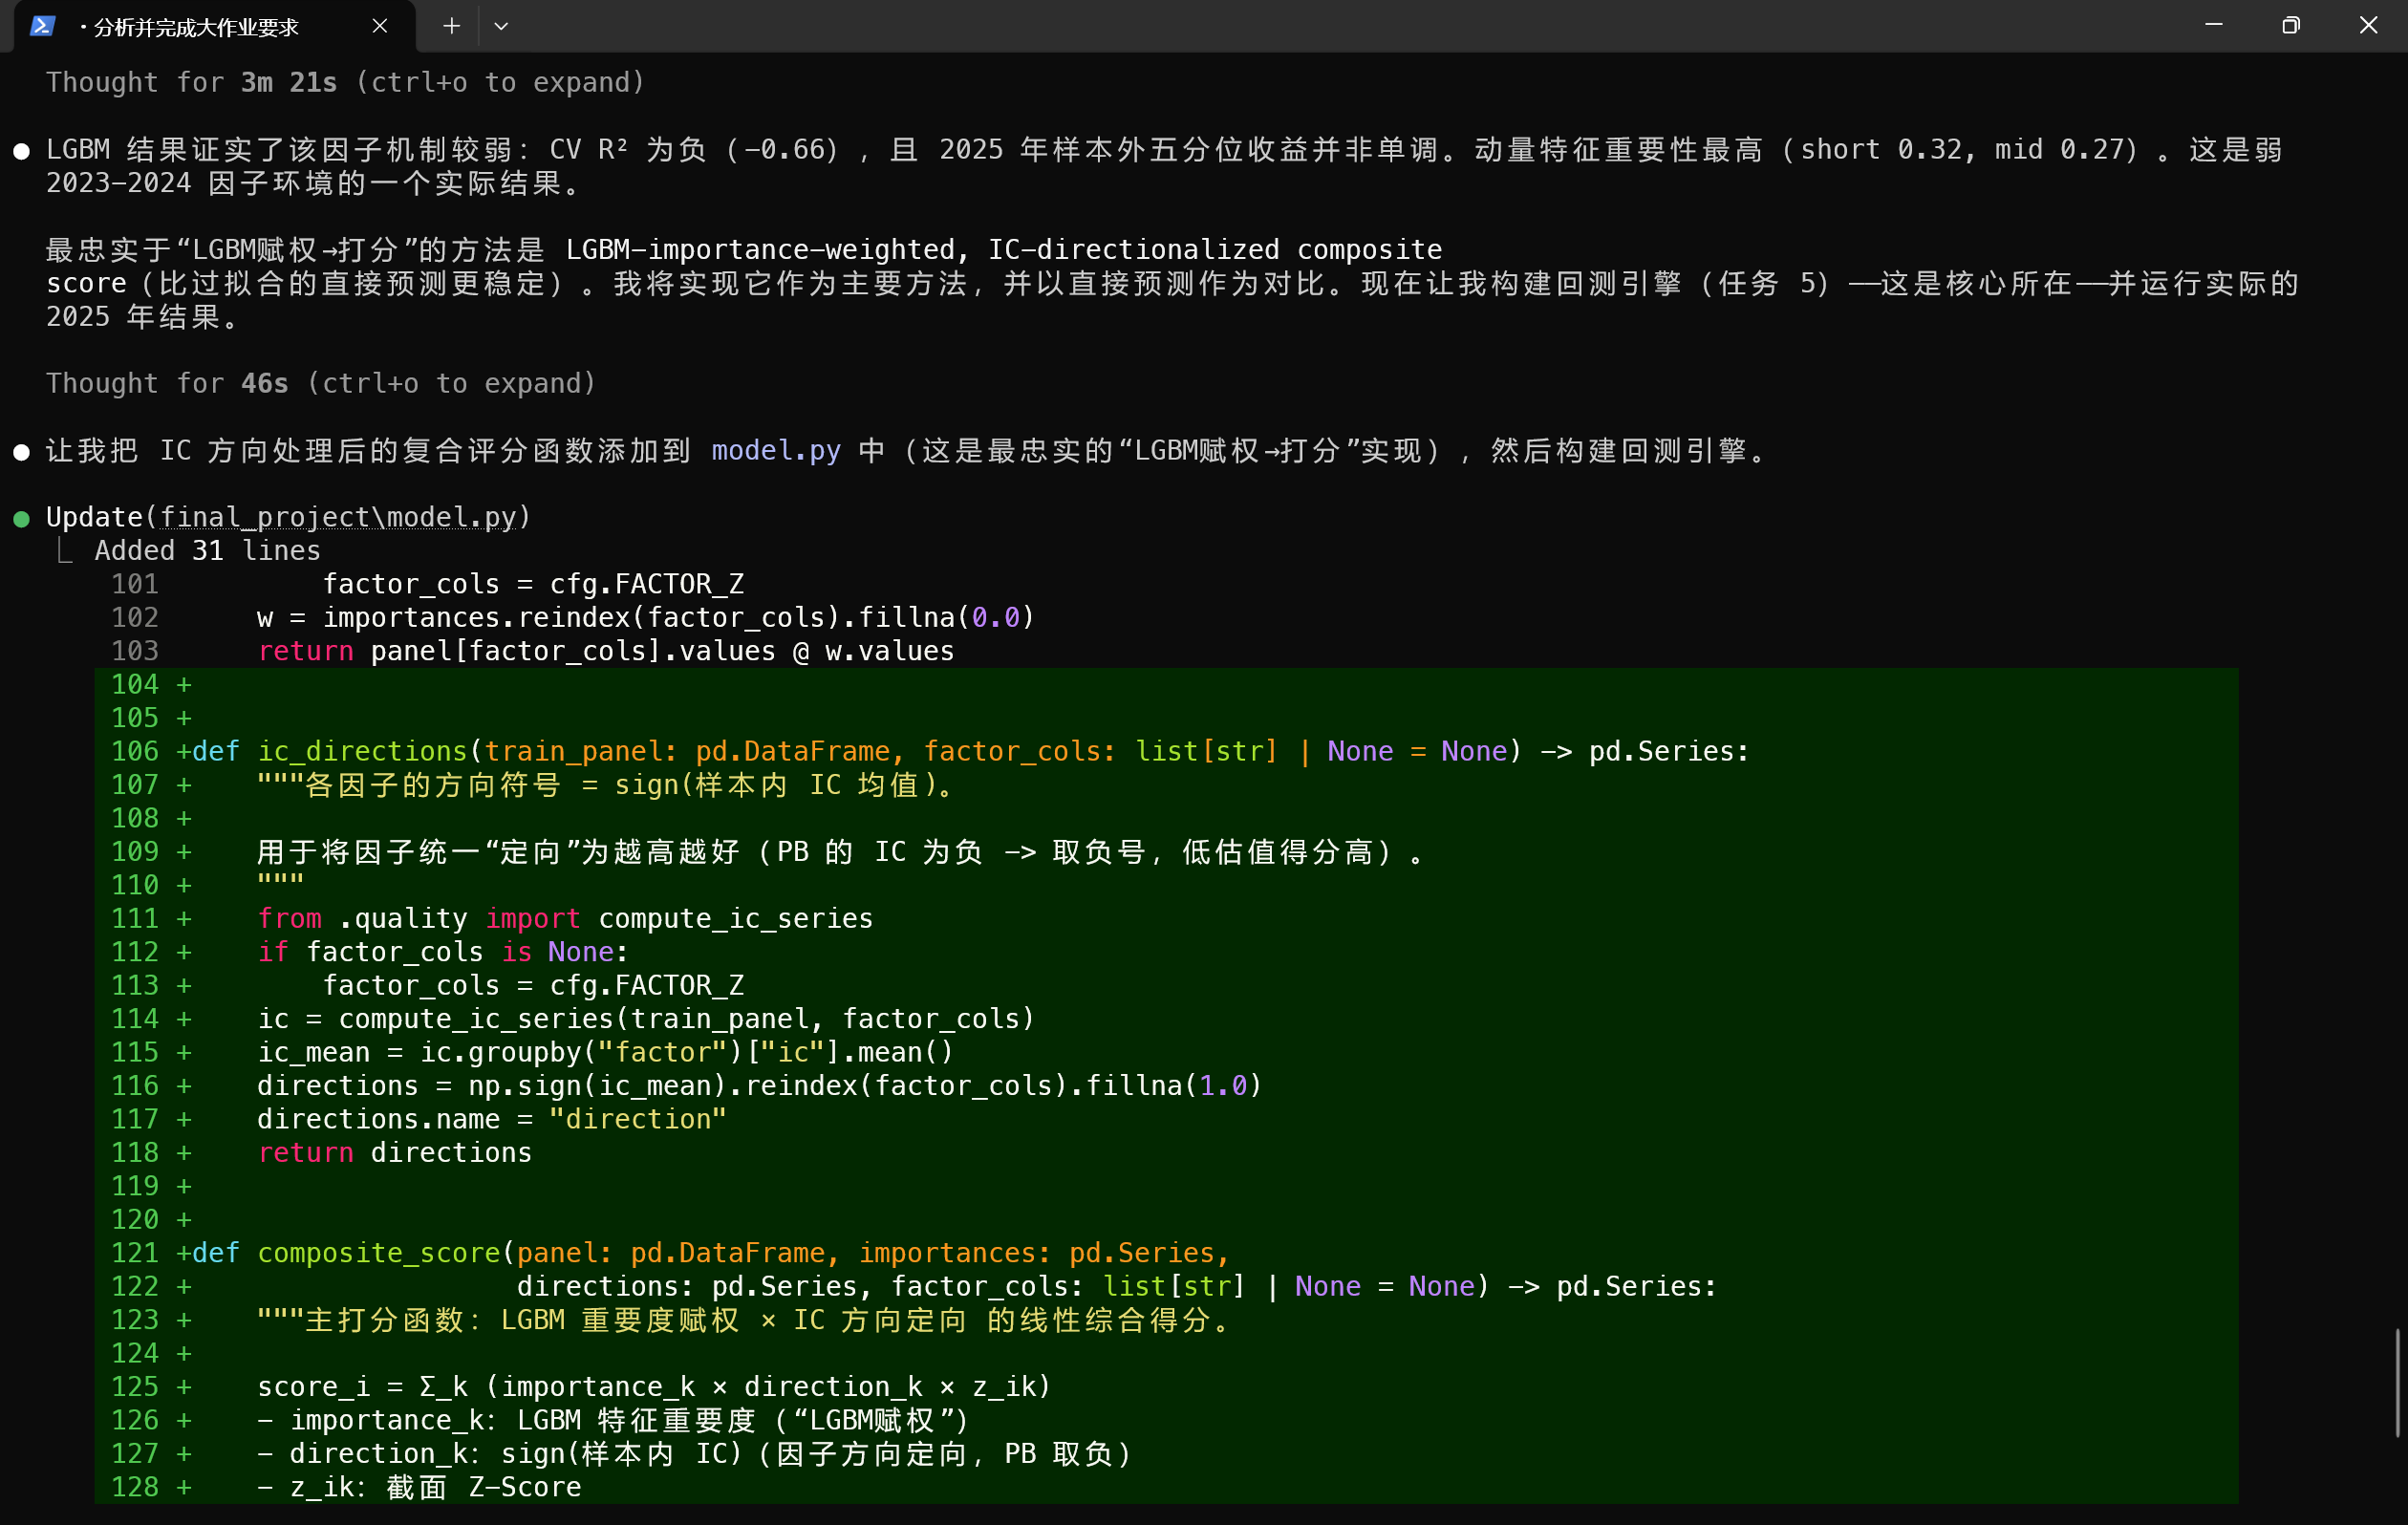
\includegraphics[width=\textwidth,height=0.82\textheight,keepaspectratio]{ai_chat_media/media/image10.png}
    \caption{AI交互记录截图（10）}
    \label{fig:ai-chat-10}
\end{figure}

\begin{figure}[p]
    \centering
    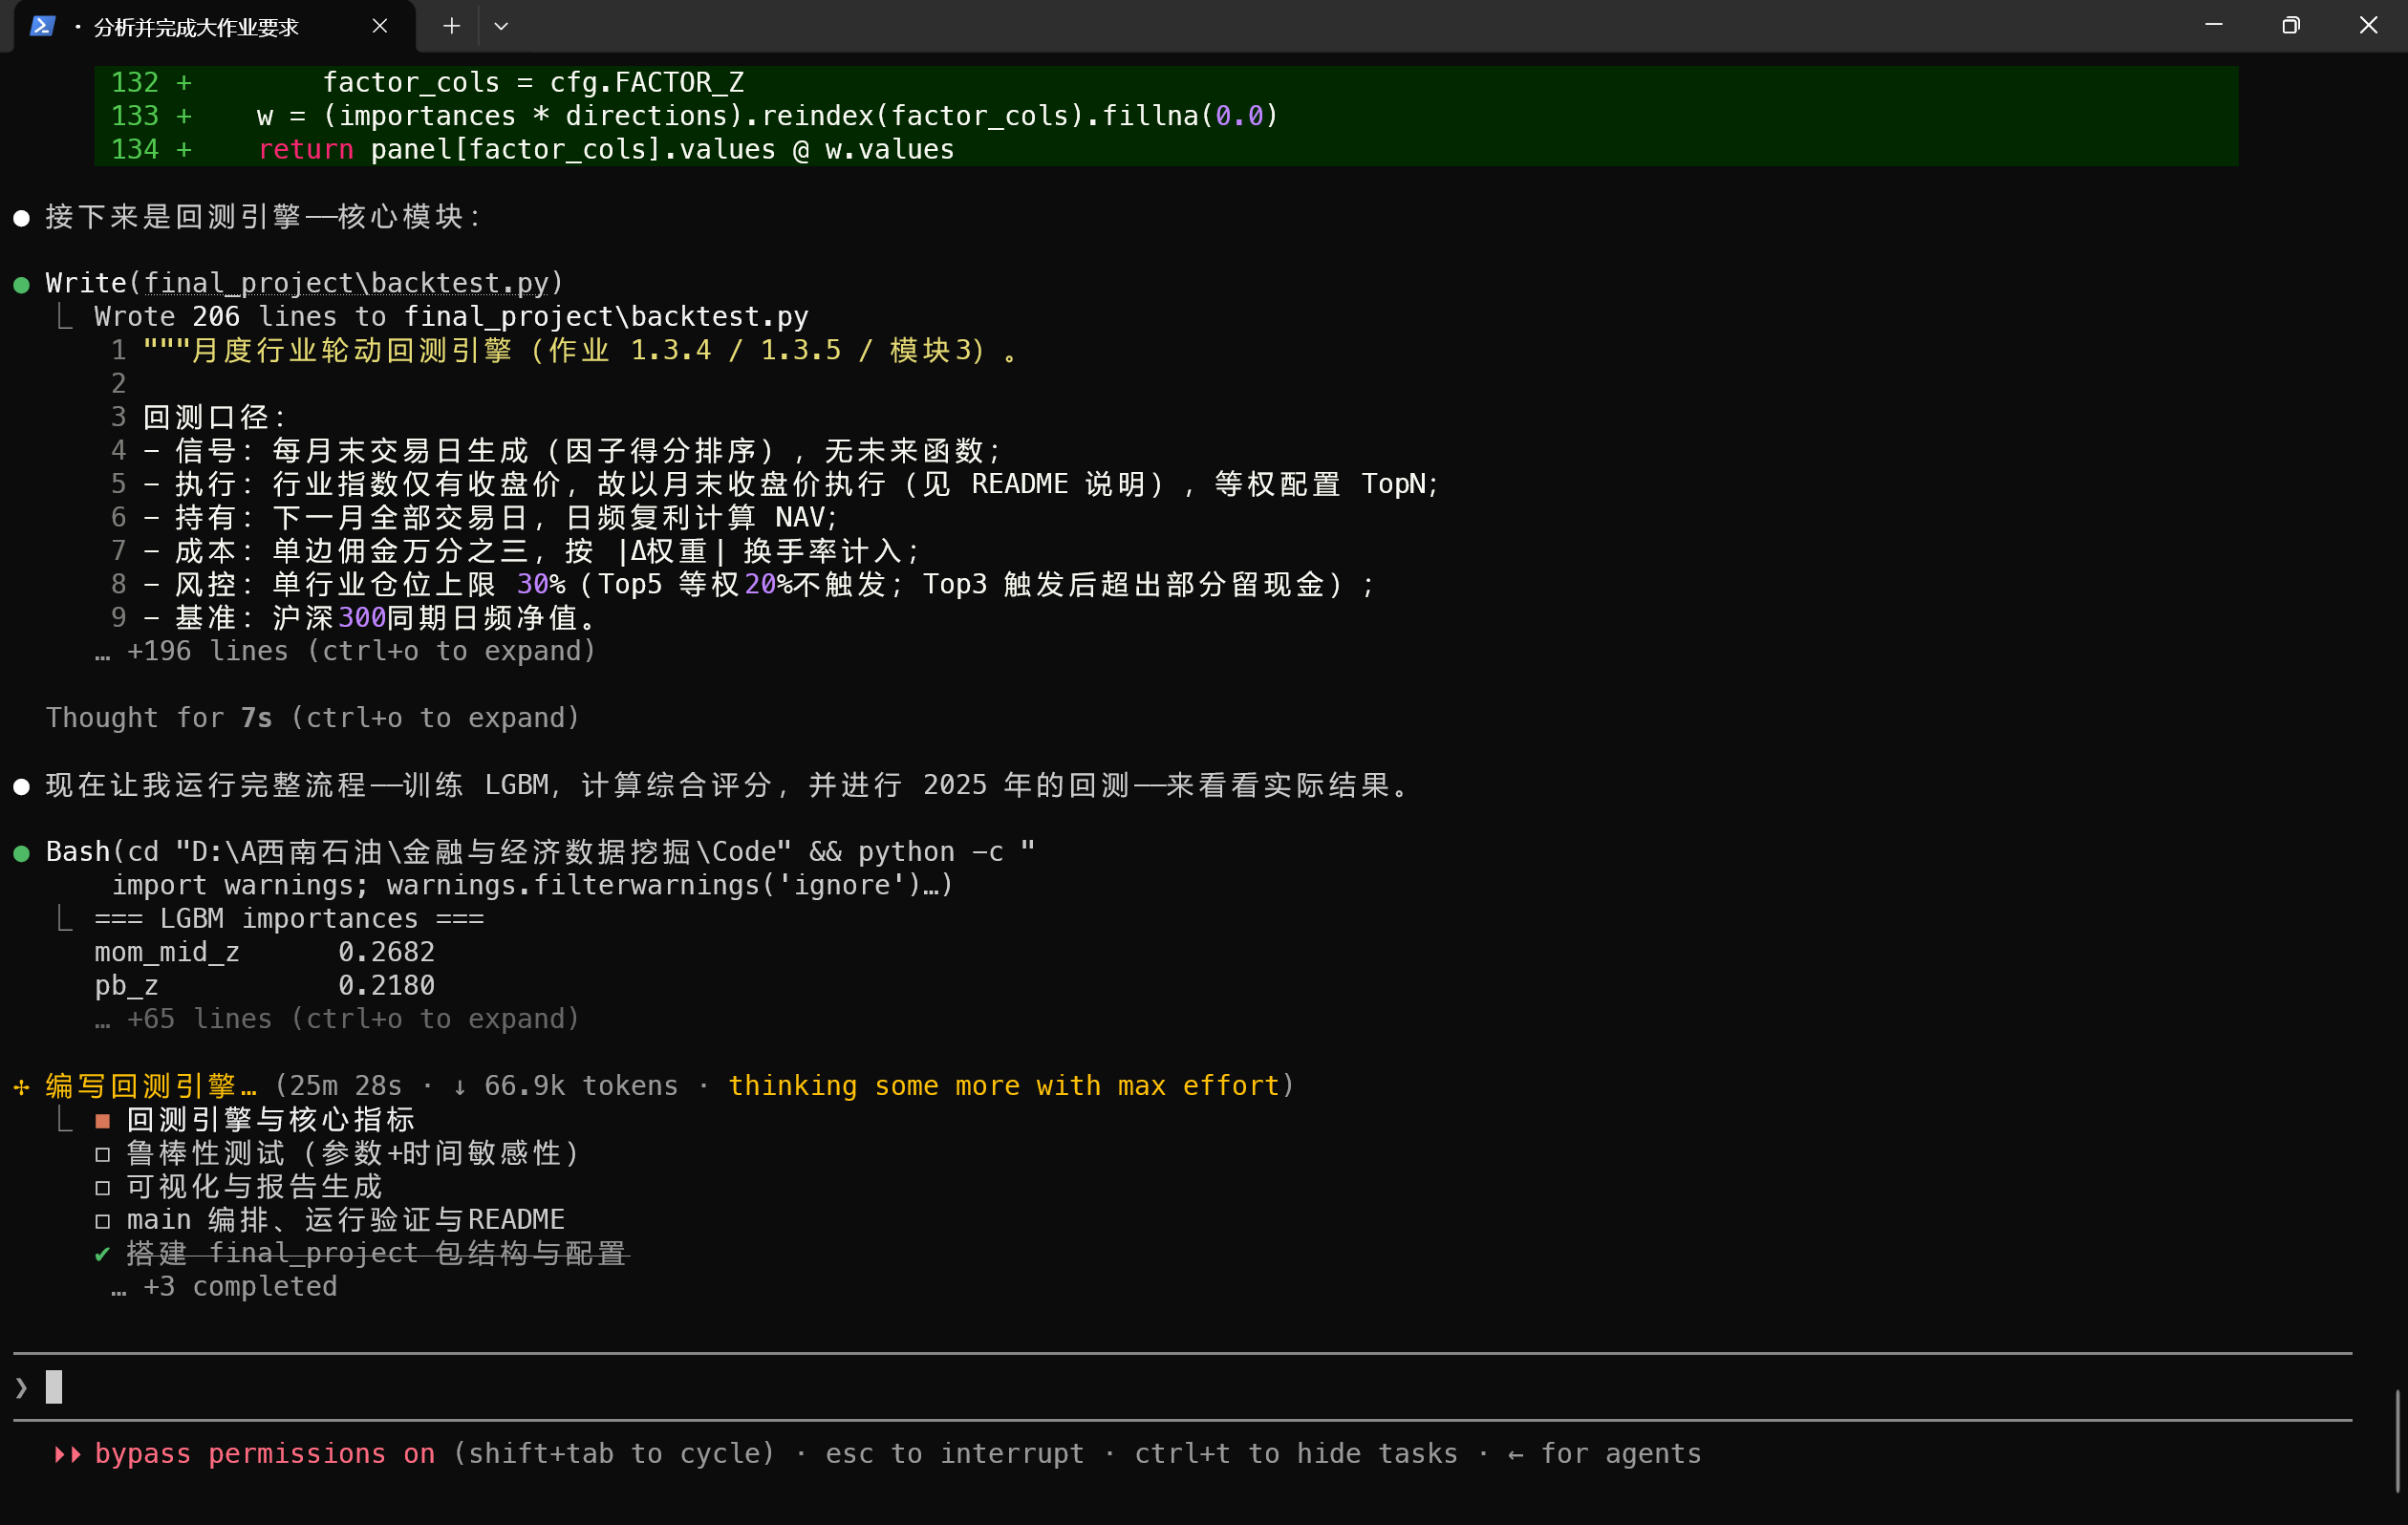
\includegraphics[width=\textwidth,height=0.82\textheight,keepaspectratio]{ai_chat_media/media/image11.png}
    \caption{AI交互记录截图（11）}
    \label{fig:ai-chat-11}
\end{figure}

\begin{figure}[p]
    \centering
    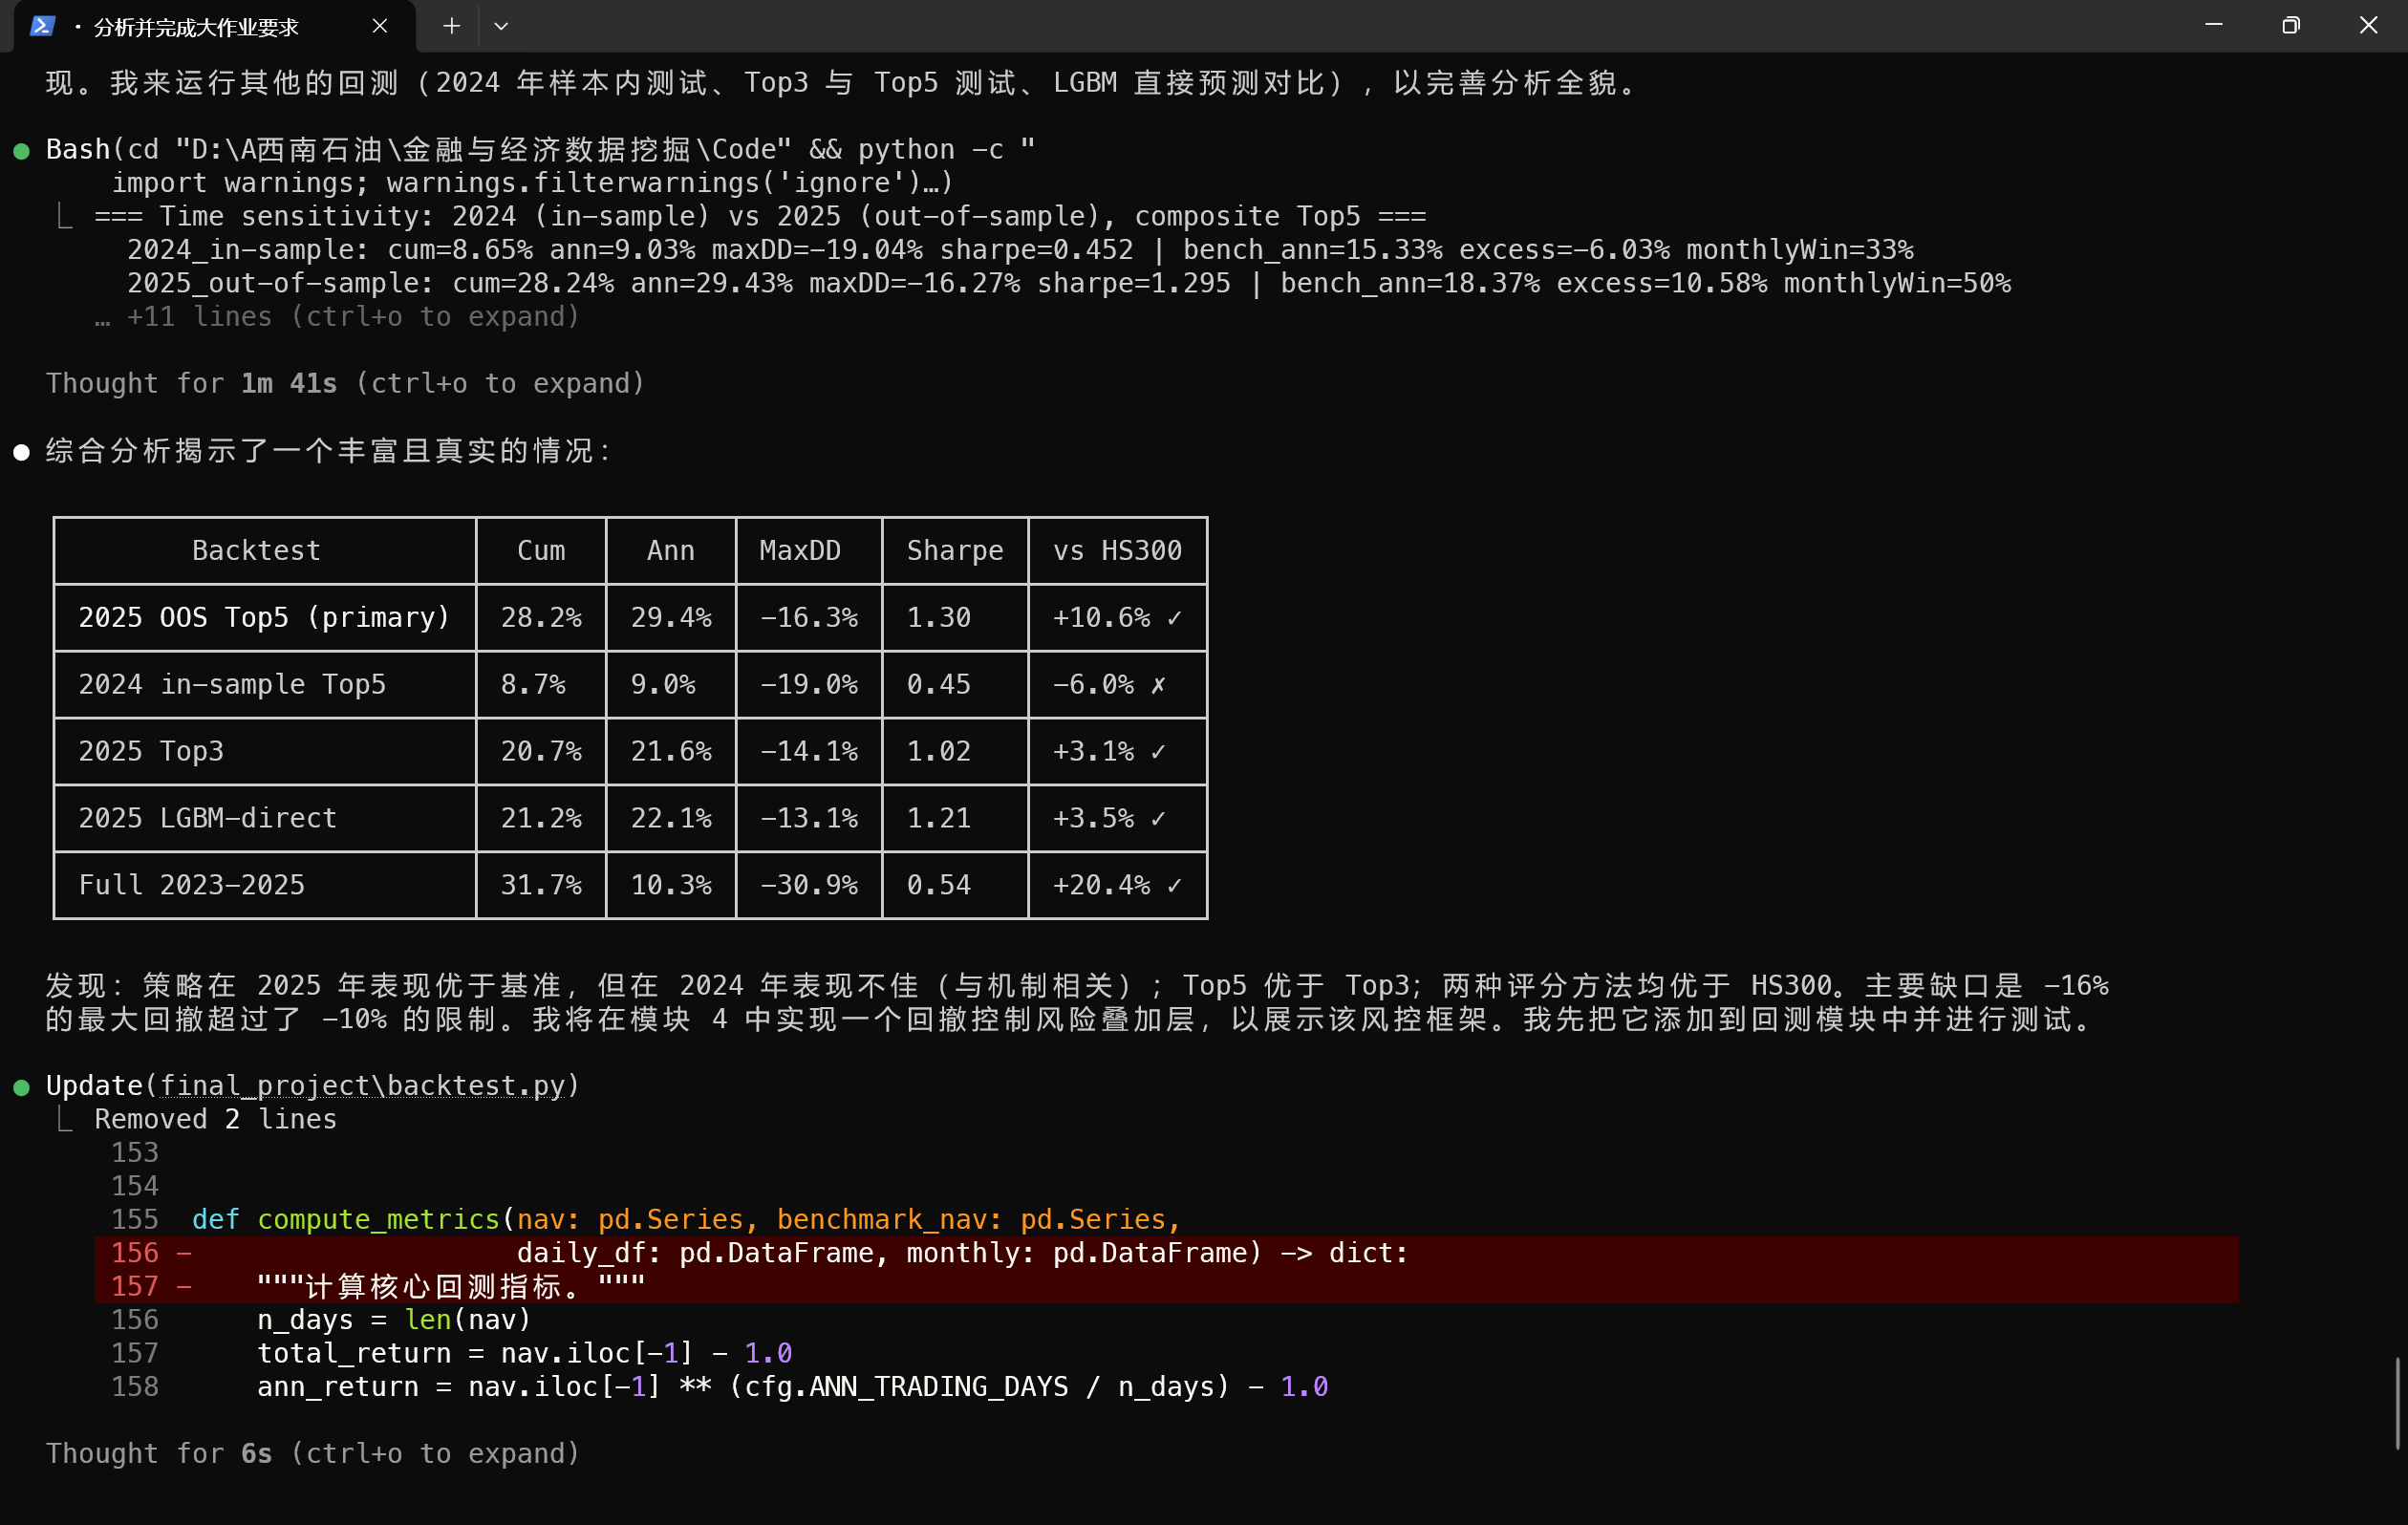
\includegraphics[width=\textwidth,height=0.82\textheight,keepaspectratio]{ai_chat_media/media/image12.png}
    \caption{AI交互记录截图（12）}
    \label{fig:ai-chat-12}
\end{figure}

\begin{figure}[p]
    \centering
    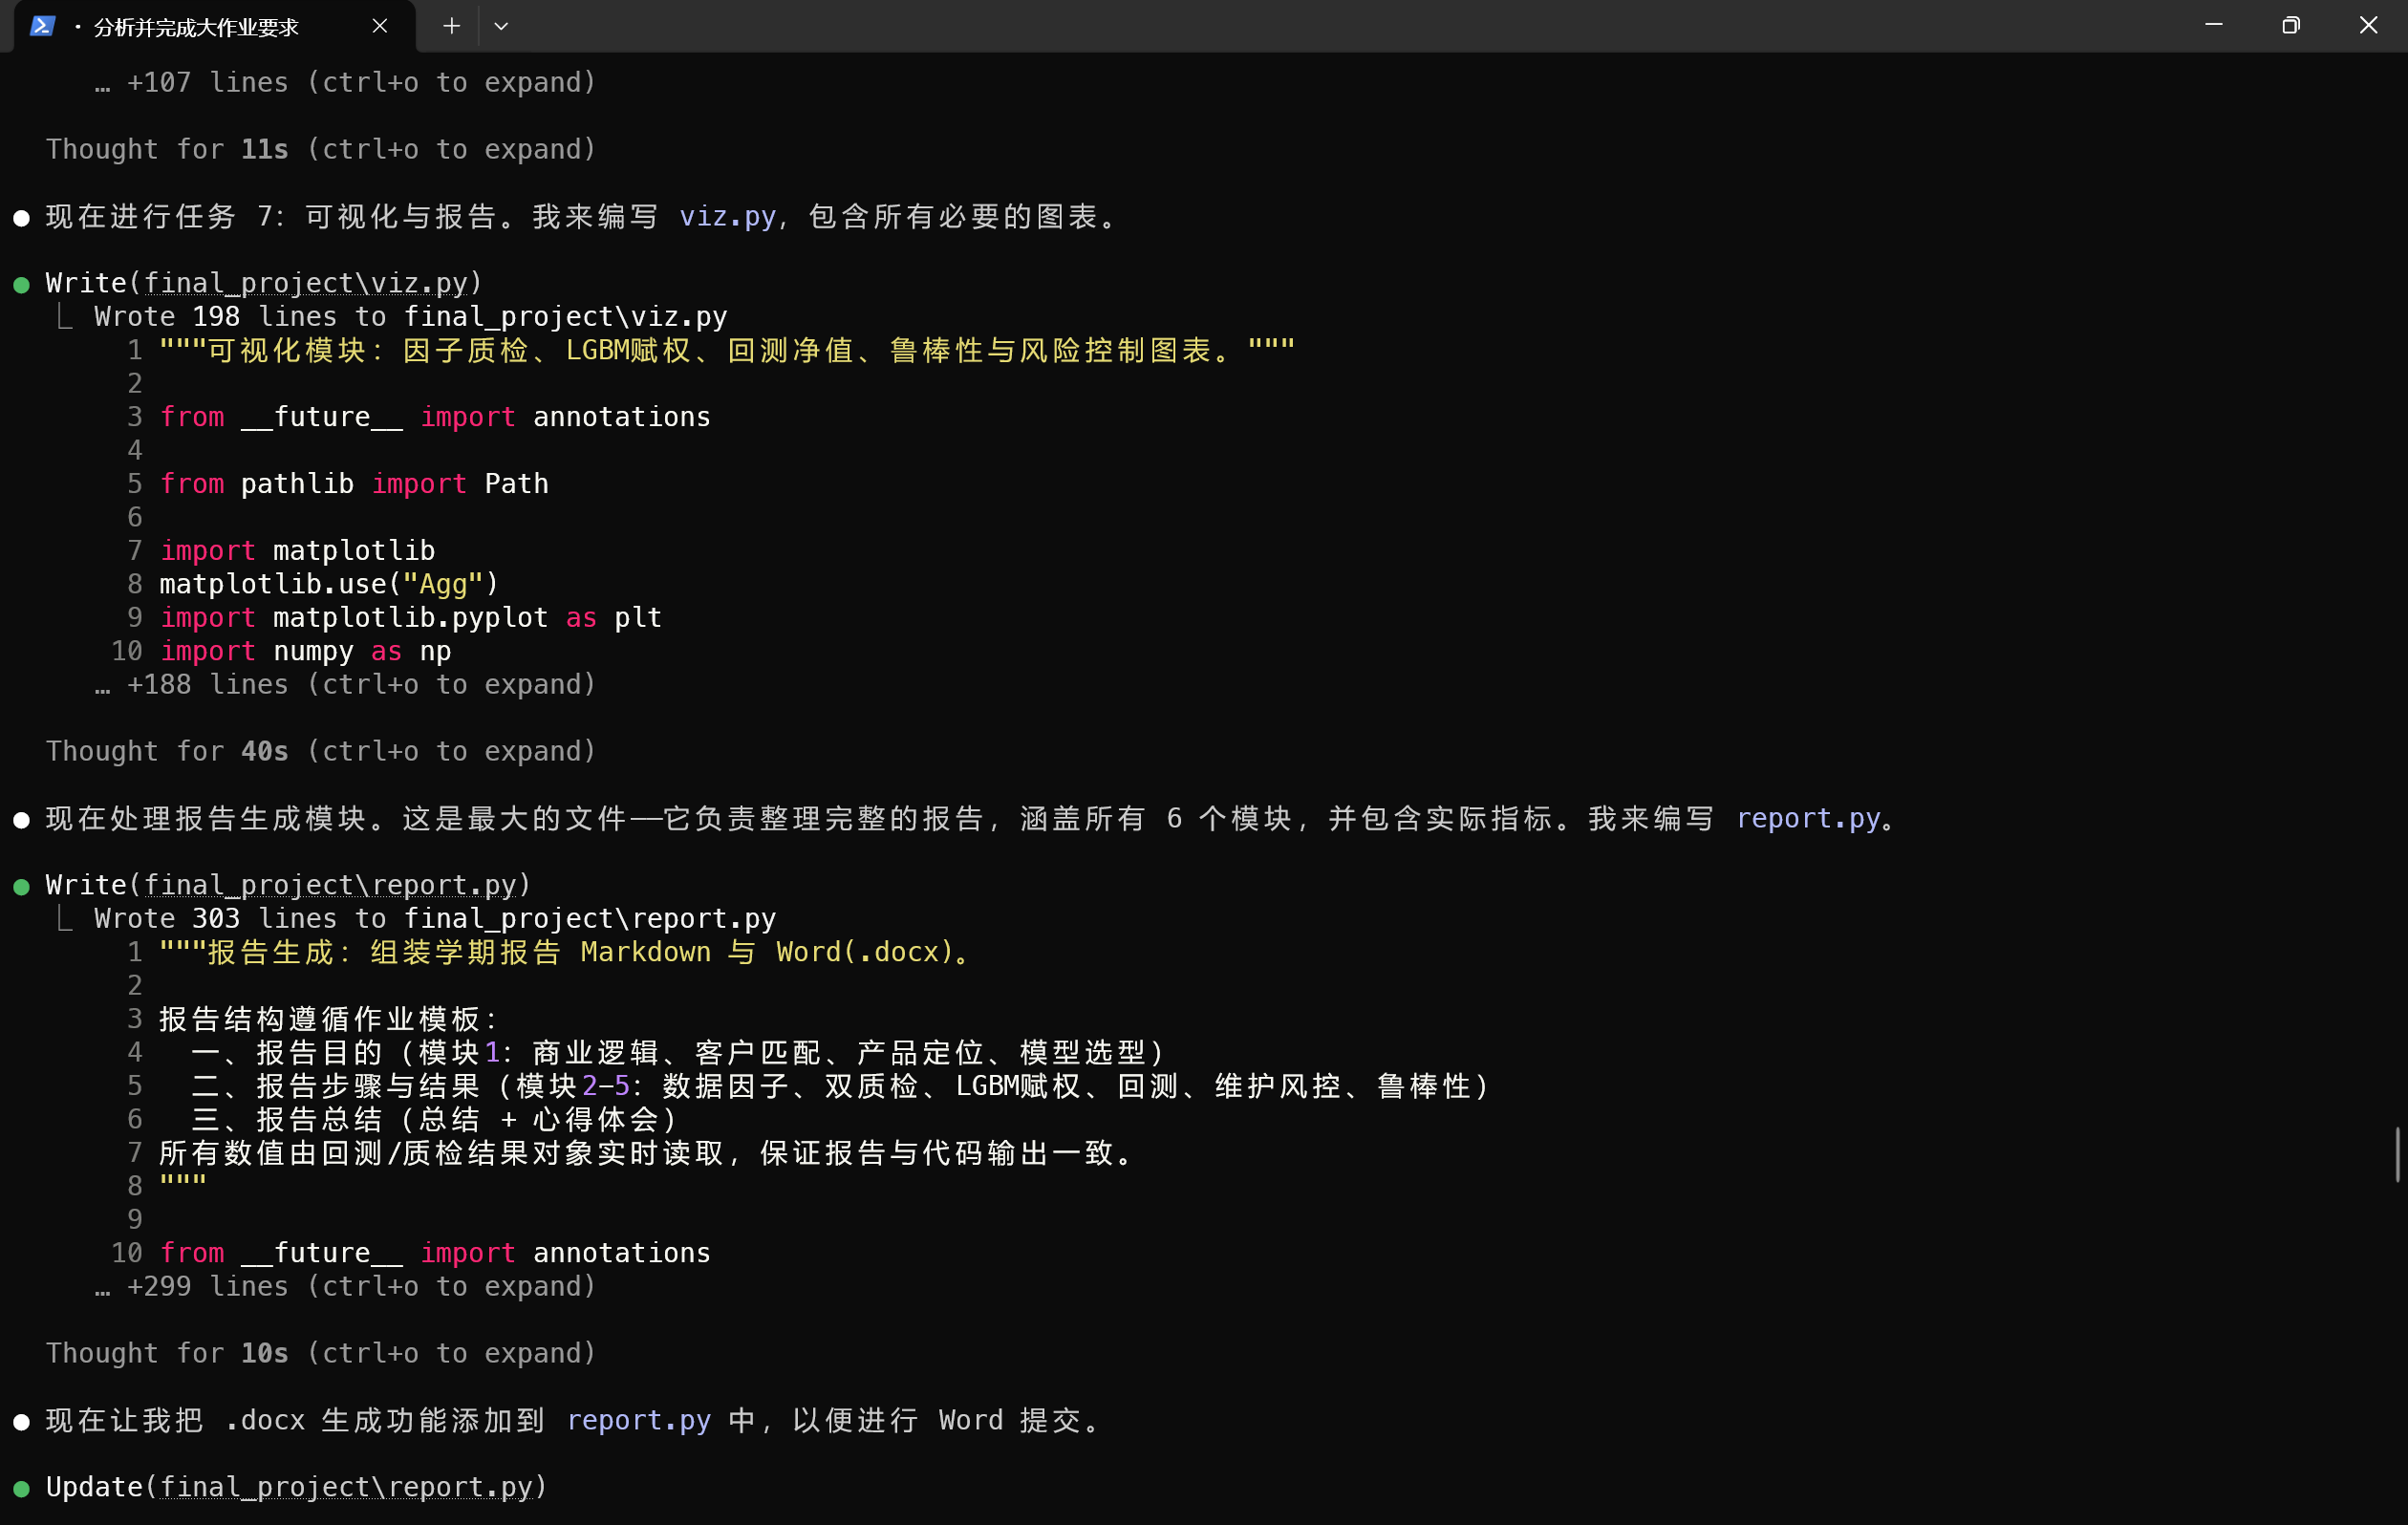
\includegraphics[width=\textwidth,height=0.82\textheight,keepaspectratio]{ai_chat_media/media/image13.png}
    \caption{AI交互记录截图（13）}
    \label{fig:ai-chat-13}
\end{figure}

\begin{figure}[p]
    \centering
    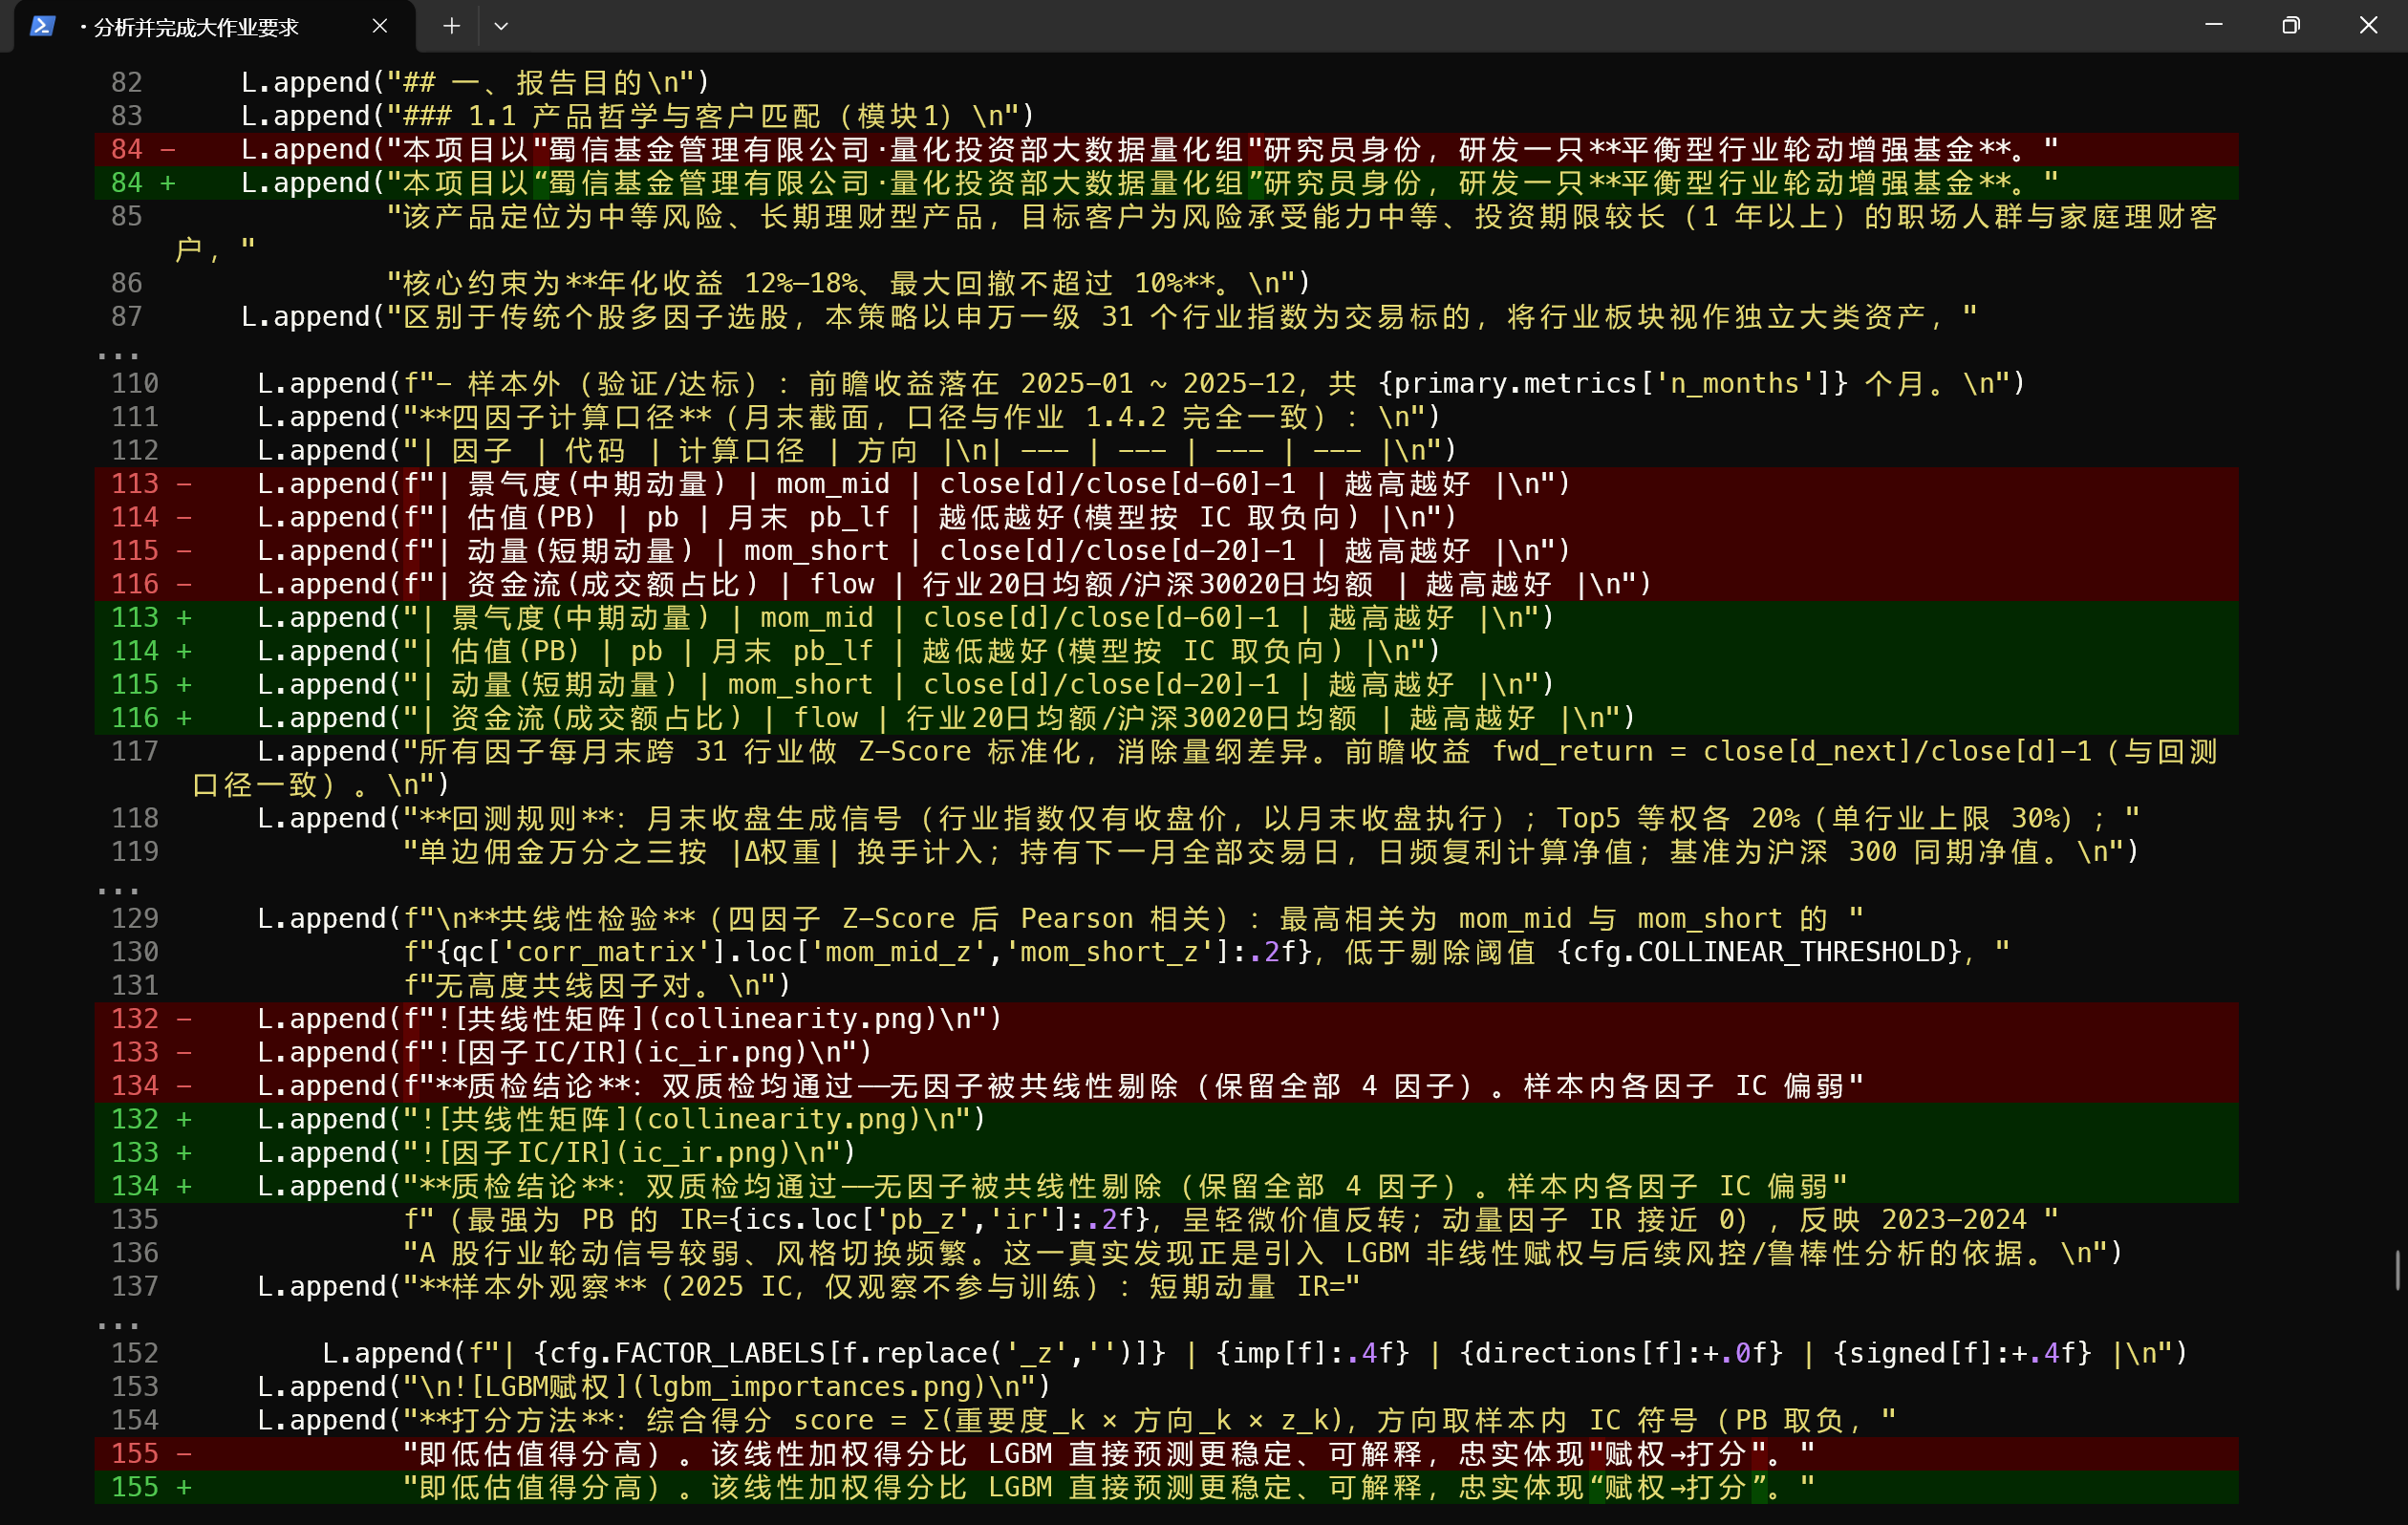
\includegraphics[width=\textwidth,height=0.82\textheight,keepaspectratio]{ai_chat_media/media/image14.png}
    \caption{AI交互记录截图（14）}
    \label{fig:ai-chat-14}
\end{figure}

\begin{figure}[p]
    \centering
    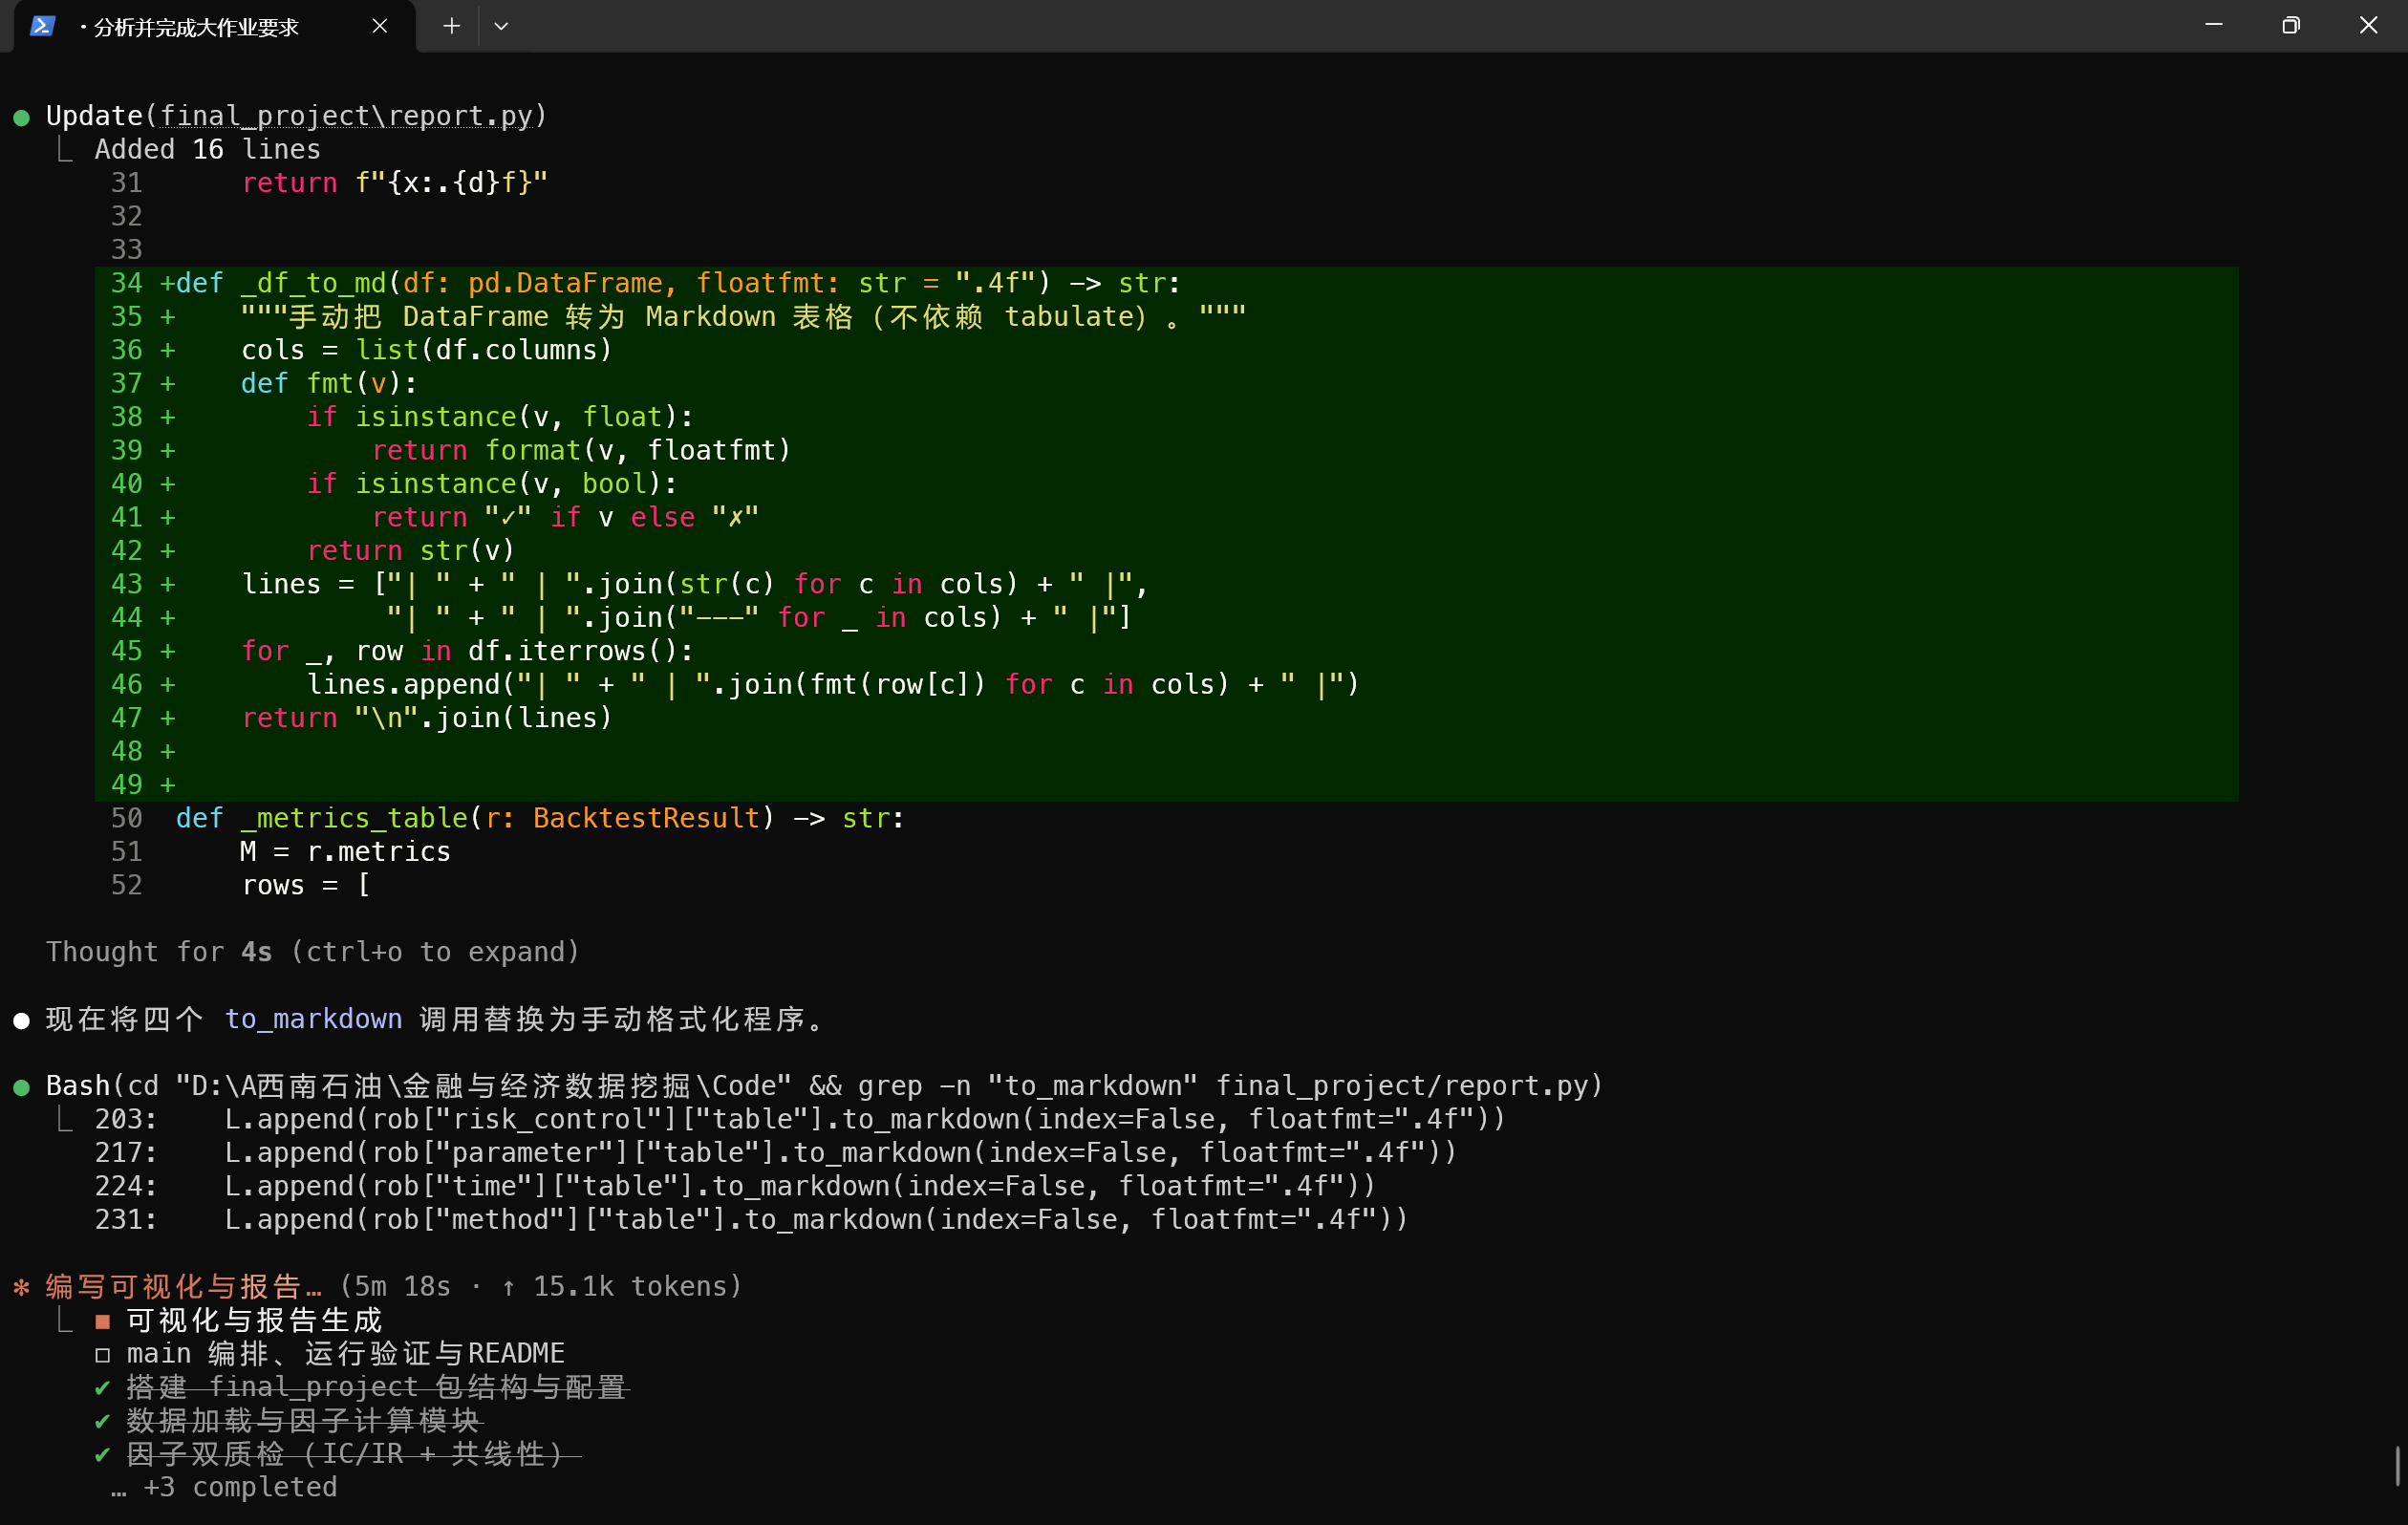
\includegraphics[width=\textwidth,height=0.82\textheight,keepaspectratio]{ai_chat_media/media/image15.png}
    \caption{AI交互记录截图（15）}
    \label{fig:ai-chat-15}
\end{figure}

\begin{figure}[p]
    \centering
    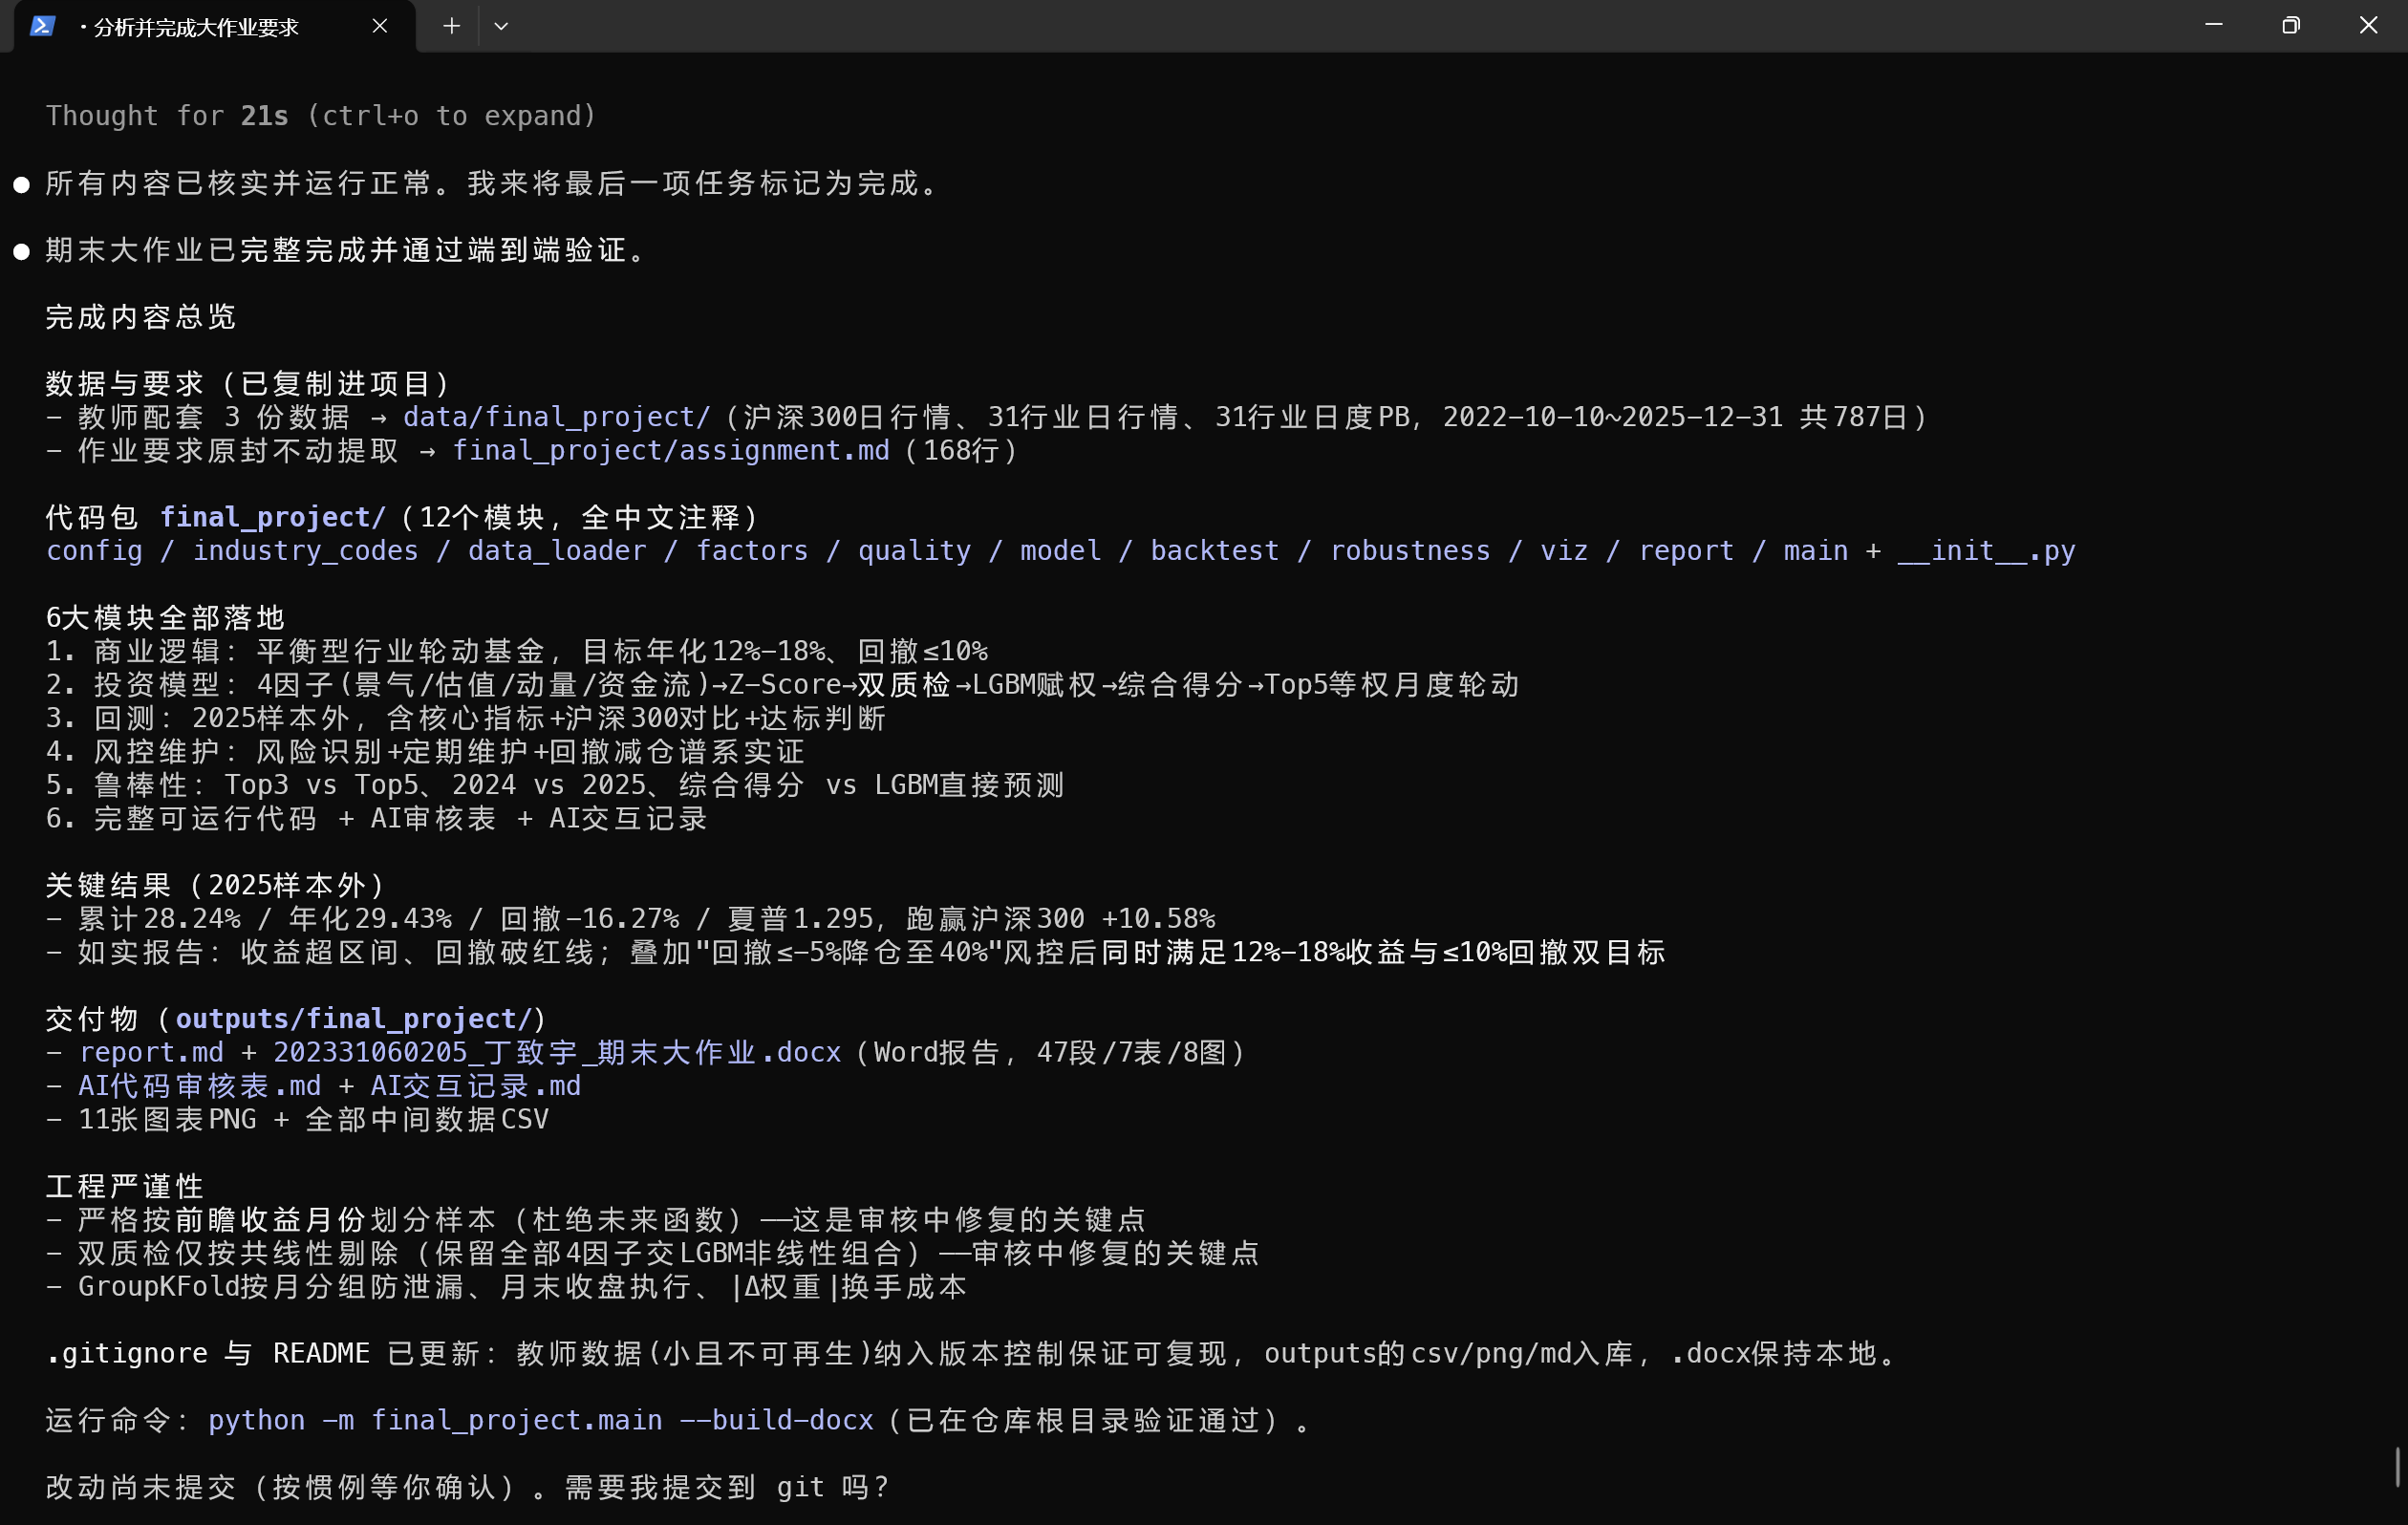
\includegraphics[width=\textwidth,height=0.82\textheight,keepaspectratio]{ai_chat_media/media/image16.png}
    \caption{AI交互记录截图（16）}
    \label{fig:ai-chat-16}
\end{figure}

\clearpage


\section{结论}

本项目完整实现了行业轮动多因子量化策略的研发流程：数据读取、因子计算、因子双质检、LightGBM 赋权、截面打分、样本外回测、风险控制、鲁棒性检验与 AI 审查记录均已落地。主策略在 2025 年样本外取得 29.62\% 累计收益和 11.96\% 累计超额，说明多因子行业轮动框架能够捕捉一定 alpha；但主策略最大回撤 -16.27\%，不符合平衡型产品定位。

最终风控版本 \texttt{trig-5\%\_exp40\%} 将年化收益控制在 14.58\%，最大回撤压至 -9.87\%，同时满足收益与回撤双目标。该结果说明，本项目不是简单追求最高收益，而是能根据产品约束对策略进行再设计和风险调校。代码审查修复也进一步提升了项目可信度，尤其是时序划分、交叉验证和风控成本三处修复，使回测结论更经得起检查。

从学习收获看，本项目最重要的体会是：金融数据挖掘中的模型准确率并不是唯一目标，时间顺序、交易成本、风险红线和报告可复现性同样决定策略是否可信。多因子模型给出投资逻辑，机器学习提供非线性赋权，风控模块负责把策略从“能赚钱”调整为“适合产品”，三者结合才是一套完整的量化研究流程。

\clearpage
\appendix
\section{核心代码附录}

以下附录收录本项目最关键的代码文件，用于证明报告结果可以从代码端复现。完整项目文件位于 \path{final_project/}，运行入口为：

\begin{CodeBlock}
python -m final_project.main --build-docx
\end{CodeBlock}

\subsection{\texorpdfstring{\texttt{config.py}}{config.py}}
\ProjectCodeInput{config.py}

\subsection{\texorpdfstring{\texttt{data\_loader.py}}{data loader.py}}
\ProjectCodeInput{data_loader.py}

\subsection{\texorpdfstring{\texttt{factors.py}}{factors.py}}
\ProjectCodeInput{factors.py}

\subsection{\texorpdfstring{\texttt{quality.py}}{quality.py}}
\ProjectCodeInput{quality.py}

\subsection{\texorpdfstring{\texttt{model.py}}{model.py}}
\ProjectCodeInput{model.py}

\subsection{\texorpdfstring{\texttt{backtest.py}}{backtest.py}}
\ProjectCodeInput{backtest.py}

\subsection{\texorpdfstring{\texttt{robustness.py}}{robustness.py}}
\ProjectCodeInput{robustness.py}

\subsection{\texorpdfstring{\texttt{main.py}}{main.py}}
\ProjectCodeInput{main.py}

\end{document}
